%%
%% This is file `sample-sigconf-authordraft.tex',
%% generated with the docstrip utility.
%%
%% The original source files were:
%%
%% samples.dtx  (with options: `all,proceedings,bibtex,authordraft')
%% 
%% IMPORTANT NOTICE:
%% 
%% For the copyright see the source file.
%% 
%% Any modified versions of this file must be renamed
%% with new filenames distinct from sample-sigconf-authordraft.tex.
%% 
%% For distribution of the original source see the terms
%% for copying and modification in the file samples.dtx.
%% 
%% This generated file may be distributed as long as the
%% original source files, as listed above, are part of the
%% same distribution. (The sources need not necessarily be
%% in the same archive or directory.)
%%
%%
%% Commands for TeXCount
%TC:macro \cite [option:text,text]
%TC:macro \citep [option:text,text]
%TC:macro \citet [option:text,text]
%TC:envir table 0 1
%TC:envir table* 0 1
%TC:envir tabular [ignore] word
%TC:envir displaymath 0 word
%TC:envir math 0 word
%TC:envir comment 0 0
%%
%% The first command in your LaTeX source must be the \documentclass
%% command.
%%
%% For submission and review of your manuscript please change the
%% command to \documentclass[manuscript, screen, review]{acmart}.
%%
%% When submitting camera ready or to TAPS, please change the command
%% to \documentclass[sigconf]{acmart} or whichever template is required
%% for your publication.
%%
%%
\documentclass[sigconf,authordraft]{acmart}


\usepackage{hyperref}
\usepackage{url}
\usepackage{amsmath,amssymb,amsfonts}
\usepackage{algorithmic}
\usepackage{graphicx}
\usepackage{textcomp}
\usepackage{xcolor}
\usepackage{pifont} % for checkmark symbol
\usepackage{threeparttable}
\usepackage{tabularx}
\usepackage{booktabs}
\usepackage{rotating}
\usepackage{wrapfig}

\usepackage{amsmath,amsfonts,amssymb,amscd,amsthm}
\usepackage{graphicx,xcolor,comment}
\usepackage{mathrsfs} 
\usepackage{calc}
\usepackage{multirow}
\usepackage{array}
\usepackage{hyperref}
\usepackage{multicol}
\usepackage{ragged2e}
\usepackage{pgfplots}
\pgfplotsset{compat=1.17}
\usetikzlibrary{pgfplots.groupplots}
% Define \sym for significance stars
\newcommand{\sym}[1]{^{#1}}
\usepackage{caption}
\usepackage[english]{babel}
\usepackage{rotating}
\usepackage{enumerate}
\usepackage{tikz}
\usepackage{bm}
\usepackage{csquotes}
\usepackage[useregional]{datetime2}
\usepackage{bbm}
\usepackage{tikz}
\usepackage{amssymb}
\usepackage{svg}
\usetikzlibrary{arrows.meta, positioning, decorations.pathreplacing}
\usepackage{amsmath}
\usepackage[export]{adjustbox}
\usepackage{mathrsfs}
\usepackage{booktabs}
\usepackage{threeparttable}
\usepackage{tabularx}
\usepackage{textcomp}
\usepackage{booktabs}
\usepackage{tabularx}
\usepackage{tikz}
\usetikzlibrary{shapes, arrows.meta, positioning, fit, backgrounds, calc, shadows}
\usetikzlibrary{shapes.geometric, arrows.meta, positioning, shadows, calc}
\usepackage{pgfplots}
\usetikzlibrary{arrows.meta, positioning, shapes.geometric}
\usepackage{amsmath}
\usepackage{tcolorbox}
\usepackage{xcolor}
\usepackage{etoolbox}
%-------- for bibliography -----------------
\usepackage{ amssymb }

\pgfplotsset{compat=1.18}

% Define colors for visual mapping
\definecolor{isoBlue}{RGB}{0, 114, 178} % Decision variables
\definecolor{costRed}{RGB}{213, 94, 0}  % Objective
\definecolor{constrGreen}{RGB}{0, 158, 115} % Constraints

% Color Scheme
\definecolor{valBlue}{RGB}{0, 114, 178}   % Value Function / Future
\definecolor{profGold}{RGB}{230, 159, 0}  % Current Profit
\definecolor{stateGray}{RGB}{100, 100, 100} % State Variables

% --- ECONOMICS STYLE DEFINITIONS ---
% Define distinct, professional colors
\definecolor{econBlue}{RGB}{0, 107, 164}  % Demand
\definecolor{econRed}{RGB}{200, 82, 0}    % Supply
\definecolor{econGreen}{RGB}{89, 89, 89}  % Old equilibrium (Neutral)
\definecolor{econGold}{RGB}{255, 128, 14} % Transmission / Action
\definecolor{econBlue}{RGB}{31, 119, 180}
\definecolor{econRed}{RGB}{214, 39, 40}
\definecolor{econGold}{RGB}{188, 143, 46}

% Consistent Color Palette
\definecolor{fossilRed}{RGB}{204, 85, 0}   % Burnt Orange for Fossil
\definecolor{reGreen}{RGB}{0, 158, 115}    % Green for Renewables
\definecolor{noteGray}{RGB}{80, 80, 80}    % For notes

\definecolor{fossilRed}{RGB}{196, 69, 54}
\definecolor{fossilRedLight}{RGB}{248, 229, 227}
\definecolor{reGreen}{RGB}{46, 125, 50}
\definecolor{reGreenLight}{RGB}{232, 245, 233}
\definecolor{primaryBlue}{RGB}{26, 54, 93}
\definecolor{primaryBlueLight}{RGB}{232, 238, 245}
\definecolor{accentOrange}{RGB}{217, 119, 6}
\definecolor{mutedGray}{RGB}{73, 80, 87}
\definecolor{surfaceGray}{RGB}{248, 249, 250}

% Define consistent styles
\tikzset{
    econAxis/.style={thick, ->, >=stealth},
    supply/.style={thick, econRed},
    demand/.style={thick, econBlue},
    priceLine/.style={thin, gray, densely dashed},
}


\usetikzlibrary{intersections, decorations.pathreplacing, arrows.meta, calc, backgrounds}

% Define consistent colors (adjust these to match your presentation theme)
\definecolor{econBlue}{RGB}{31, 119, 180}
\definecolor{econRed}{RGB}{214, 39, 40}
\definecolor{econGold}{RGB}{188, 143, 46}

% Define consistent styles
\tikzset{
    econAxis/.style={thick, ->, >=stealth},
    supply/.style={thick, econRed},
    demand/.style={thick, econBlue},
    priceLine/.style={thin, gray, densely dashed},
}

%%
%% \BibTeX command to typeset BibTeX logo in the docs
\AtBeginDocument{%
  \providecommand\BibTeX{{%
    Bib\TeX}}}

%% Rights management information.  This information is sent to you
%% when you complete the rights form.  These commands have SAMPLE
%% values in them; it is your responsibility as an author to replace
%% the commands and values with those provided to you when you
%% complete the rights form.
\setcopyright{acmlicensed}
\copyrightyear{2018}
\acmYear{2018}
\acmDOI{XXXXXXX.XXXXXXX}
%% These commands are for a PROCEEDINGS abstract or paper.
\acmConference[Conference acronym 'XX]{Make sure to enter the correct
  conference title from your rights confirmation email}{June 03--05,
  2018}{Woodstock, NY}
%%
%%  Uncomment \acmBooktitle if the title of the proceedings is different
%%  from ``Proceedings of ...''!
%%
%%\acmBooktitle{Woodstock '18: ACM Symposium on Neural Gaze Detection,
%%  June 03--05, 2018, Woodstock, NY}
\acmISBN{978-1-4503-XXXX-X/2018/06}
\bibliographystyle{ACM-Reference-Format}


%%
%% Submission ID.
%% Use this when submitting an article to a sponsored event. You'll
%% receive a unique submission ID from the organizers
%% of the event, and this ID should be used as the parameter to this command.
%%\acmSubmissionID{123-A56-BU3}

%%
%% For managing citations, it is recommended to use bibliography
%% files in BibTeX format.
%%
%% You can then either use BibTeX with the ACM-Reference-Format style,
%% or BibLaTeX with the acmnumeric or acmauthoryear sytles, that include
%% support for advanced citation of software artefact from the
%% biblatex-software package, also separately available on CTAN.
%%
%% Look at the sample-*-biblatex.tex files for templates showcasing
%% the biblatex styles.
%%

%%
%% The majority of ACM publications use numbered citations and
%% references.  The command \citestyle{authoryear} switches to the
%% "author year" style.
%%
%% If you are preparing content for an event
%% sponsored by ACM SIGGRAPH, you must use the "author year" style of
%% citations and references.
%% Uncommenting
%% the next command will enable that style.
%%\citestyle{acmauthoryear}


%%
%% end of the preamble, start of the body of the document source.
\begin{document}

%%
%% The "title" command has an optional parameter,
%% allowing the author to define a "short title" to be used in page headers.
\title{An Econometric Model for Measuring System-level impacts of AI on United States Power Grids}

%%
%% The "author" command and its associated commands are used to define
%% the authors and their affiliations.
%% Of note is the shared affiliation of the first two authors, and the
%% "authornote" and "authornotemark" commands
%% used to denote shared contribution to the research.
\author{Dana Golden}
% \authornote{Both authors contributed equally to this research.}
\email{dana.golden@stonybrook.edu}
\orcid{1234-5678-9012}
\affiliation{%
  \institution{Stony Brook University School of Economics}
  \city{Stony Brook}
  \state{New York}
  \country{USA}
}

\author{Aruna Balasubramanian}
\affiliation{%
  \institution{Stony Brook University School of Computer Science}
  \city{Stony Brook}
  \country{New York}}
\email{arunab@cs.stonybrook.edu}

\author{Niranjan Balasubramanian}
\affiliation{%
  \institution{Stony Brook University School of Computer Science}
  \city{Stony Brook}
  \country{New York}}
\email{niranjan@cs.stonybrook.edu}



%%
%% By default, the full list of authors will be used in the page
%% headers. Often, this list is too long, and will overlap
%% other information printed in the page headers. This command allows
%% the author to define a more concise list
%% of authors' names for this purpose.
\renewcommand{\shortauthors}{Golden, Balasubramanian, Balasubramanian}

%%
%% The abstract is a short summary of the work to be presented in the
%% article.
\begin{abstract}
Data centers are a major source of power demand growth in the 21st century. Artificial Intelligence has accelerated this trend with power demand by data centers growing from 1.9\% of total US power demand to 4.4\% of US power in only six years. While anecdotal evidence suggests that AI data centers are using enough power to have substantial impacts on the U.S. power grids, there are no systematic studies to quantify these effects. We utilize econometric techniques to determine the impact of AI model training and inference on consumer electricity quality and fossil fuel power demand. We find significant reductions in power quality and significant increases in power demand near data centers both immediately before and immediately after the publication of AI models. The largest impact worsens power quality equivalent to an additional .5-1 power outages per year. We further show these estimates can also be used for counterfactual analysis to assess impacts of scaling for future model development. 
\end{abstract}

%%
%% The code below is generated by the tool at http://dl.acm.org/ccs.cfm.
%% Please copy and paste the code instead of the example below.
%%
\begin{CCSXML}
<ccs2012>
 <concept>
  <concept_id>10010520.10010553.10010562</concept_id>
  <concept_desc>Computer systems organization~Embedded and cyber-physical systems</concept_desc>
  <concept_significance>500</concept_significance>
 </concept>
 <concept>
  <concept_id>10010520.10010553.10010559</concept_id>
  <concept_desc>Computer systems organization~Reliability</concept_desc>
  <concept_significance>300</concept_significance>
 </concept>
 <concept>
  <concept_id>10010405.10010489</concept_id>
  <concept_desc>Applied computing~Energy management systems</concept_desc>
  <concept_significance>300</concept_significance>
 </concept>
 <concept>
  <concept_id>10010147.10010257</concept_id>
  <concept_desc>Computing methodologies~Machine learning</concept_desc>
  <concept_significance>100</concept_significance>
 </concept>
</ccs2012>
\end{CCSXML}

\ccsdesc[500]{Computer systems organization~Embedded and cyber-physical systems}
\ccsdesc[300]{Computer systems organization~Reliability}
\ccsdesc[300]{Applied computing~Energy management systems}
\ccsdesc[100]{Computing methodologies~Machine learning}

%%
%% Keywords. The author(s) should pick words that accurately describe
%% the work being presented. Separate the keywords with commas.
\keywords{Artificial intelligence, power grids, electricity markets, reliability, power quality, econometrics}
%% A "teaser" image appears between the author and affiliation
%% information and the body of the document, and typically spans the
%% page.
% \begin{teaserfigure}
%   
\includegraphics[width=\textwidth]{sampleteaser}
%   \caption{Seattle Mariners at Spring Training, 2010.}
%   \Description{Enjoying the baseball game from the third-base
%   seats. Ichiro Suzuki preparing to bat.}
%   \label{fig:teaser}
% \end{teaserfigure}

\received{20 February 2007}
\received[revised]{12 March 2009}
\received[accepted]{5 June 2009}

%%
%% This command processes the author and affiliation and title
%% information and builds the first part of the formatted document.
\maketitle

\section{introduction}

\begin{wrapfigure}{r}{0.45\linewidth}
    \centering
    \vspace{-10pt}
    
\includegraphics[width=.8\linewidth]{Figures/Data Center Electricity Consumption over Time (1).jpg}
    \caption{Projected data center growth over time. Source: DOE.}
    \label{fig:DataCenterGrowth}
    \vspace{-10pt}
\end{wrapfigure}

Over the past six years, data centers have expanded from consuming 1.9\% to 4.4\% of total U.S. electricity demand (Figure \ref{fig:DataCenterGrowth}, DOE). This rapid growth—driven largely by artificial intelligence—follows two decades of flat electricity consumption and coincides with nationwide efforts to electrify transport and heating. Together, these trends are straining the power grid and raising concerns about both reliability and affordability. Recent anecdotal evidence, such as \cite{Nicoletti_Malik_Tartar_2024}, points to data centers reducing local power quality and raising prices. 


However, systematic empirical evidence on these power-grid impacts remains scarce. Existing techno-economic assessments such as those from international organizations, and industry-focused reports~\cite{RN1, RN3} broadly highlight increasing share of AI workloads in the data center market. At the micro-level, some studies examine the energy performance of different AI accelerators and identify workload management opportunities for reducing power consumption\cite{RN9} and \cite{RN4}. Last, a vast body of computer science literature focuses on the compute, energy, and environmental costs of AI model development and deployment~\cite{strubell19,schwartz2020green,RN7, RN5, morrison2025holistically}. While these provide a strong basis for understanding how AI models impact datacenter level demand and efficiency opportunities, in this work we ask questions about the impact at the power-grid level with implications for energy reliability and security. %See~\autoref{sec:related-work} for a broader discussion.


%Energy consumption of AI models has received a lot of attention for its financial and environmental costs~\cite{} .  At a micro level, the AI community uses estimates of energy consumption of AI models for an instance and extrapolates to a data center level and the consequent environmental impacts (e.g. carbon footprints, embodied emissions) of training and deploying such models~\cite{}. At a macro level, the proliferation of data centers (e.g. DOE data shows demand rose from 1.9\% to 4.4\% of total U.S. electricity as in Figure \ref{fig:DataCenterGrowth}, DOE) and the ever increasing AI workloads in these, pose tremendous challenges to the power grids themselves. The huge loads cause fluctuations affecting power quality, and increasing demands, in conjunction with the increasing demand for renewables. 

Understanding these power grid level impacts is critical from the perspectives of energy reliability and security. In this paper, we ask seek to answer three specific questions: 1) What are the effects of AI model releases on local power quality and power frequency? 2) How do AI training and inference affect electricity consumption around data centers owned by model developers? 3) How to analyze these grid impacts under counterfactual scenarios of efficiency and model use?

It is challenging, however, to quantify these \emph{macro} grid-level impacts of AI models due to the lack of fine-grained data about other contributing factors that are unobservable due to proprietary aspects or otherwise prohibitively expensive to obtain. For example the power quality of a grid can be affected by many external factors including seasonal trends, location effects and data center internal factors such as other workloads which are unobservable proprietary information. 

We employ econometric Difference-in-Differences (DiD) models to quantify the causal effects of AI model deployments on power systems. By comparing data centers running AI models against control groups of random data centers, and partitioning observations into pre- and post-model release periods, we isolate the impact of AI deployments while controlling for temporal and geographic factors. Using publicly available data on datacenter locations, power grids, AI model releases, weather, and market prices, we find that large AI models cause significant power quality deterioration (exceeding half the standard deviation of US power-quality distributions) and increase fossil fuel demand by terawatt hours---\textbf{equivalent to powering 100,000 homes annually}---during both training and inference phases. These estimates enable counterfactual projections for evaluating different scenarios' effects on energy consumption and grid stability.

We apply this methodology using publicly available market data on datacenter locations, power grid information, AI model release times, and other appropriate control data (e.g. weather, market prices). Specifically, we learn these DiD regressors for predicting measures of both power quality and demand. 
We find that large models cause significant power quality deterioration in nearby areas (well above half the standard deviation of US power-quality distributions), and increase fossil fuel demand in the order of terrawatt hours (equivalent to powering 100K homes a year) in both training and inference. We also show how these estimates can be used to evaluate different scenarios, enabling counterfactual projections of their effects on energy consumption and grid stability. 

In summary, this work contributes (i) a methodology for assessing and monitoring the macro impacts of AI models on the power grid even when specific fine-grained data maybe unavailable, and (ii) the first quantitative estimates of these macro grid-level impacts of some major frontier models, adding complementary evidence to the emerging literature on the environmental and system-level impacts of AI data centers \cite{murino2023sustainable,guidi2024environmental,thangam2024impact}. 

%Over the past six years, data centers have expanded from consuming 1.9\% to 4.4\% of total U.S. electricity demand (Figure \ref{fig:DataCenterGrowth}, DOE). This rapid growth—driven largely by artificial intelligence—follows two decades of flat electricity consumption and coincides with nationwide efforts to electrify transport and heating. Together, these trends are straining the power grid and raising concerns about both reliability and affordability. Recent anecdotal evidence, such as \cite{Nicoletti_Malik_Tartar_2024}, points to data centers reducing local power quality and raising prices. Yet, systematic empirical evidence on these impacts remains scarce.

 %\aruna{we should align this with the three questions we ask in Section 4}

%To answer these questions, we combine econometric analysis of market data with techno-economic modeling of AI workloads. This dual approach allows us to move beyond carbon-intensity metrics and instead provide the first empirical estimates of AI’s impact on electricity demand and power quality near data centers. We then link these estimates to technical scenarios of AI efficiency gains, enabling counterfactual projections of their effects on energy consumption and grid stability. In doing so, our work contributes to the emerging literature on the environmental and system-level impacts of AI data centers \cite{murino2023sustainable,guidi2024environmental,thangam2024impact}, offering new insights into both environmental quality and energy security.

% The paper is organized as follows. Section 1 reviews the literature related to data center power usage. Section 2 describes the structure of the data center market and presents descriptive statistics power consumption by data centers and the impact of AI on data center power consumption. Section 3 presents a model of data center power procurement while Section 4 describes the methodology for the estimation of models related to answering the research question. Section 5 provides a description on results and model-fit. Section 6 details counterfactuals related to the impact of reducing AI power consumption on power quality. Section 7 details future research and concludes the paper.



\section{Background: Datacenter Concentration and Power-Quality}
The U.S. data centers are expanding rapidly, nearly tripling from its 2008 levels to 1489 active sites in 2025, with another 1,359 on the horizon~\cite{aterio_us_data_centers_2025}. The market is dominated by \emph{hyperscalers}---vertically integrated datacenters---owned by AI heavy companies such as Amazon, Microsoft, and Google, alongside a long tail of smaller operators. Hyperscalers afford companies certain economies of scale but greatly increase the geographic concentration of power demand on the grids. Concentrated demand strains local grids in the area, raising congestion costs and sometimes degrading power quality for neighboring consumers. Large, inflexible loads from AI hyperscalers also reduce system reliability, elevate wholesale prices, and complicate renewable integration.
%\niranjan{These paragraphs can be compressed to state the problem more succinctly. Datacenters are concentrated in geographic locations because they provide certain benefits that come from economies of scale. This while has some economic benefits also brings in infrastructural impacts. We could even change the title of the section to: Background: Datacenter Concentration and Power-Quality Impact. End this section with questions on what to do about this.}
%\niranjan{Then move the Data sub-section to Methodology Section.}
%\subsection{Market Overview}

%The U.S. data center market has expanded rapidly, growing from 519 facilities in 2008 to 1,489 active sites in 2025, with another 1,359 announced or under construction \cite{aterio_us_data_centers_2025}. Electricity demand more than tripled over this period, rising from under 5 to over 15 GWh per hour (BNEF), while total U.S. capacity increased only 17.6\% \cite{EIA_2023_table4_2A} and dispatchable baseload capacity fell as coal retired.
% \niranjan{Renewable generation is not something we touch upon in the rest of the paper. Should we drop this reference? It would be better to talk about power generation and power demand in general.}
% Power consumption has risen in parallel, though since 2018 growth in renewable generation has outpaced data center demand as shown in Figure \ref{fig:DCPowerConsumption}.

% \begin{wrapfigure}{l}{0.45\linewidth}
%     \centering
%     \vspace{-10pt}
%     
\includegraphics[width=\linewidth]{Figures/Data Center Power Demand vs Green Generation.png}
%     \caption{Data center power consumption vs.\ green generation. Source: Aterio.io.}
%     \label{fig:DCPowerConsumption}
%     \vspace{-10pt}
% \end{wrapfigure}

%The market is geographically concentrated and dominated by hyperscalers—Amazon, Microsoft, and Google—who account for 38\% of capacity across five firms, and 64\% across twenty. Unlike colocation providers such as Equinix, hyperscalers are vertically integrated, owning facilities, long-term power contracts, fiber networks, and custom chips. These economies of scale lower costs but also create externalities: concentrated demand strains local grids, elevates congestion, and reduces reliability, though clustering also generates jobs, tax revenue, and services. Given hyperscalers’ role in AI training and their outsized grid impacts, our analysis focuses on them.


% \begin{figure}[t!]
%     \centering
%     % First figure
%     \begin{minipage}[t]{0.45\linewidth}
%         \centering
%         
\includegraphics[width=\linewidth]{Figures/Data Centers by State.png}
%         \caption{Data centers by state. Source: Aterio.io. \niranjan{Dont think this picture contributes much to the discourse. Move to appendix for space.}}
%         \label{fig:DCbyState}
%     \end{minipage}
%     \hfill
%     % Second figure
%     \begin{minipage}[t]{0.45\linewidth}
%         \centering
%         
\includegraphics[width=\linewidth]{Figures/HarmonicDistortion.png}
%         \caption{Total harmonic distortion representation.}%\aruna{this figure is not referenced in the text}}        
%         \label{fig:THD}
%     \end{minipage}
%     \vspace{-2.05em}
% \end{figure}

% These economies of scale, however, generate externalities. Concentrated demand in specific regions strains local grids, raising congestion costs and sometimes degrading power quality for neighboring consumers. Large, inflexible loads reduce system reliability, elevate wholesale prices, and complicate renewable integration. At the same time, clustering provides local benefits through jobs, tax revenues, and downstream services. Data centers thus act as both efficiency drivers and sources of regional externalities. It is important to consider the mitigation of the externalities to the grid when analyzing the impacts of AI. We focus on hyperscalers in our paper because hyperscalers perform the majority of AI training and also because larger facilities are more likely to cause power distortions.
%\aruna{Is there a reason why we are talking about hyperscalers? Should we say therefore we focus on these hyperscalers?}

AI workloads affect power quality through three main mechanisms. First, data centers and AI computing facilities add substantial baseload demand that can strain grid capacity and compromise voltage regulation, especially during peak periods. Second, AI workloads fluctuate rapidly with computational needs, creating unpredictable load variations that challenge stability and frequency regulation. Third, the switching power supplies and electronics essential to AI hardware generate harmonic distortion, introducing waveform distortions that spread through distribution networks and degrade power quality. See Figure \ref{fig:THD} in Appendix for an illustration of this harmonic distortion.

% The industry is also geographically concentrated. Texas, California, and especially Virginia dominate U.S. capacity. Virginia’s cluster reflects historic federal investments in internet infrastructure and the routing of early traffic through Northern Virginia. More recent growth in Texas stems from lower electricity costs and streamlined permitting.

% The electricity market includes three separate components: generation, transmission, and distribution. Generation is how power is produced. Transmission involves long-range transportation of electricity while distribution involves local distribution of electricity. In the United States, there are two primary models of how the electricity market is structured: vertically integrated utilities and deregulated markets. In vertically integrated utilities, which are prevalent in the South and West, generation, distribution, and transmission are all owned and operated by one company whereas in deregulated markets generation bids in wholesale markets to provide power to utilities, which own transmission and distribution, and provide power in the retail markets. Figure \ref{fig:ISOMap} provides a map showing the geographic makeup of the American electricity market.

% \begin{figure}
%     \centering
%     
\includegraphics[width=0.5\linewidth]{Figures/ISOMap.png}
%     \caption{Map of American electricity market.}
%     \label{fig:ISOMap}
% \end{figure}

These dynamics interact with broader shifts in the electricity market: greater electrification and the transition from fossil fuels to renewables. Because renewables are intermittent and less dispatchable, rising data center loads coupled with greater renewable penetration place dual pressures on grids, shaping both market outcomes and policy debates. It is therefore crucial to quantify how much power AI uses, how it distorts quality, and the role of efficiency improvements.
\section{Methodology}

\subsection{Problem}

%\niranjan{Change the questions to reflect the three main questions we currently have. Power quality and distortion are now just one question. Add the question about the efficiency counterfactual.}
We analyze three primary effects of artificial intelligence (AI) data centers on the power market, with a focus on how their presence and operations interact with grid stability and demand. 

First, we consider the effects of AI models on the index of power quality and power frequency distortions in the vicinity of data centers. Power quality reflects the stability and reliability of the grid, particularly in terms of voltage and frequency deviations. The intensive and often irregular power draw of data centers—especially during periods of large-scale training runs—can generate fluctuations that degrade local power quality. Frequency stability is a central component of reliable electricity supply, and distortions can indicate imbalances between supply and demand. Because AI training loads are highly concentrated in time and location, they may create stress points in the grid that elevate the risk of such distortions. 
 
 To this end, we evaluate whether the deployment of new frontier models, which require extraordinary computational resources, coincides with measurable declines in regional power quality indices, thereby signaling potential challenges for grid operators. Similarly, by linking model release timelines to observed patterns in frequency deviations, we assess the extent to which the roll-out of individual models exacerbates local power quality issues beyond baseline fluctuations.

Second, we consider the effects of both training and inference workloads on overall power demand in the vicinity of data centers. Training runs, while episodic, are energy-intensive and can produce sharp spikes in consumption, whereas inference tends to generate a steadier but still substantial level of ongoing demand. Both activities alter local load profiles, raising questions about the adequacy of transmission capacity, the role of long-term contracts for renewable energy procurement, and the broader implications for regional electricity markets. By distinguishing between training and inference, we highlight how different stages of the AI lifecycle place unique and evolving pressures on power systems.

Finally, we provide analysis of the impacts of improvements in AI efficiency on power quality and power demand nearby to data centers. AI efficiency broadly defined represents improvements that can be made to reduce the energy required by models without significant corresponding decreases in quality. AI efficiency represents the main lever computer scientists have at their disposal to reduce the power consumption of AI models. We utilize our econometric estimates to determine real-world impact and combine with experimental data on the effects of hardware choices for AI to extrapolate lab estimates to meaningful impact.



\subsection{Econometric Model}

Quantifying these effects is difficult given limited data on key variables. To overcome this, we draw on econometric methods, which allow credible inference even when proprietary data are unavailable. \begin{wrapfigure}{r}{0.45\linewidth}
    
    \vspace{-10pt} % adjust vertical position relative to the text
    \centering
    
\includegraphics[width=0.98\linewidth]{Figures/gblog-difference-in-differences-march-2019.png}
    \caption{Difference-in-differences estimation visualized.}
    \label{fig:DIDFigure}
    \vspace{-10pt} % tighten space below caption
\end{wrapfigure}
For example, \citet{hausman1997valuation} infers telecom demand from price and quantity variation, \citet{fowlie2012industrial} evaluate environmental regulation in electricity using emissions and price data, and \citet{card1994minimum} study minimum wage effects via cross-state employment variation. Similarly, \citet{greenstone2014environmental} analyze Indian pollution policy using ambient monitors rather than industry disclosures. These show that when markets transmit the mechanisms of interest, public data can yield the only feasible evidence. Our study follows this tradition: by exploiting observable shifts in prices, load, and capacity, we infer data center impacts that would otherwise remain opaque.


%\niranjan{Can we make this a more forceful paragraph by showing other solid papers that use this type of methodology? The following paragraph shows one paper, but lets add use cases where this is the only feasible approach.}
The particular econometric tool we use to analyze the impacts of specific AI models is \textit{Difference-in-Differences} (DiD). Originally popularized in empirical economics through applications such as \cite{card2022design} on training programs and \cite{card1994comment} on minimum wages, difference-in-differences has become one of the most widely used methods for causal inference with observational data. The technique estimates treatment effects by comparing the change in outcomes over time for a treated group to the change for a control group, as illustrated in Figure~\ref{fig:DIDFigure}. In our application, this translates to estimating the change in generator-level power demand within a ten--square--mile radius of a data center before and after the release of a major AI model. Formally, we estimate
\begin{equation}
    Y_{it} = \alpha + \beta \,(\text{Treatment}_i \times \text{Post}_t) + \gamma_i + \delta_t + \varepsilon_{it},
    \label{eq:DiD}
\end{equation}
where $Y_{it}$ is power demand for generator $i$ at time $t$, $\text{Treatment}_i$ indicates proximity to a data center, and $\text{Post}_t$ captures periods after the release of a major AI model. The coefficient of interest, $\beta$, measures the causal impact of model releases on local power demand. By differencing across both groups and periods, DiD controls for unobserved factors that are constant over time or shared across groups, with validity relying on the ``parallel trends'' assumption. The data learns the coefficient of interest by taking the difference between the average change from the initial baseline between treated and untreated regions. %\niranjan{Mention how the data is used to learn/estimate the co-efficients.}
%\niranjan{Add an equation here and refer to it in the text above.}

% \end{figure}
\subsection{Power Quality Model}
%\niranjan{Refer to the equations in the text.}
To analyze the effects of data centers on local power quality, we conduct two primary statistical analyses. First, we draw on Whisker Labs’ measures of power quality and total harmonic distortion (THD) to estimate difference-in-differences regressions that capture the impact of AI model releases. For example, if Meta were to release a new model at a specific data center, and this activity had a causal effect on nearby power quality, we would expect to observe greater deterioration in local indices relative to areas not exposed to the release. The difference-in-differences framework allows us to test precisely this comparison by linking data on data center locations, AI model release dates, and retail electric authority service areas with Whisker Labs’ measures. DiD methodology also allows us to control for sources of endogeneity. See Section \ref{sectionData} for more details on the data used.
%\niranjan{Say saomething like for example if Meta releases a model in a datacenter x if this were to have a causal impact on the local power quality, we would expect to see more deterioriations in the power quality in this locality compared to deteriorations in other areas or measures. The diff-in-diff apporach we detail below helps us measure this impact} 
%\niranjan{Add forward pointer.}

% \niranjan{Use the treatment post observation terminology to explain how this specific causal inference is done for the effects of AI model releases on power quality.}
Our econometric framework uses a standard difference-in-differences design to estimate the causal effects of AI model releases on grid quality. Regions with model launches serve as the \textbf{treatment group}, while those without form the \textbf{control group}. The \textbf{pre-treatment period} is the six months before a release, and the \textbf{post-treatment period} is the six months after. For demand regressions, we shorten the window to three months given the higher granularity and longer time series of the demand dataset. By contrast, power quality data are more limited, so we cannot run pre-treatment regressions, though robustness checks for alternative time intervals are provided in the appendix.
%\dana{I will add these robustness checks. Ultimately, the main reason for the 3 month six month change was that it's easier to identify an effect with a smaller interval, and that works better with hourly data by generator than monthly data by utility. We can definitely play around with this though.} \niranjan{why is it that we do pre and post treatment only for power demand and not for power quality impact? and why six months here and why three months for power demand?}

As shown in Equation~\ref{eq:powerquality}, we model the effect on the Consumer Power Quality Index, while Equation~\ref{eq:thd} examines total harmonic distortion. 

\begin{equation}
\text{PowerQuality}_{rt} = \alpha 
+ \beta \left( \text{Post}_{t} \times \text{Treatment}_{r} \right)
+ \gamma_r + \delta_t + \varepsilon_{rt}
\label{eq:powerquality}
\end{equation}
\begin{equation}
\text{TotalHarmonicDistortion}_{rt} = \alpha' 
+ \beta' \left( \text{Post}_{t} \times \text{Treatment}_{r} \right)
+ \gamma'_r + \delta'_t + \varepsilon'_{rt}
\label{eq:thd}
\end{equation}

The key interaction term $\text{Post}_{t} \times \text{Treatment}_{r}$ captures the difference between treatment and control regions in the post-treatment period relative to the pre-treatment period. This double-differencing approach allows us to isolate the causal effect of AI model launches by controlling for: (1) time-invariant regional characteristics through region fixed effects $\gamma_r$ (or $\gamma'_r$), and (2) common temporal trends affecting both treatment and control regions through time fixed effects $\delta_t$ (or $\delta'_t$). 

The estimated coefficients $\beta$ and $\beta'$ therefore represent the average treatment effect---the causal impact of AI model releases on power quality and harmonic distortion in treatment regions during the post-treatment observation period, net of what would have occurred absent the AI launch.



\subsection{Power Demand Model}

Power demand is a composite over fossil fuels, nuclear, and other renewables. Here we focus on fossil fuel demand partly because we have access to the necessary generator-level data and to avoid additional complexities that arise in modeling nuclear and renewable demands\footnote{It is common in economic analyses to focus on fossil fuel demand in part because renewable generation is unresponsive to demand shocks}.%\niranjan{Add renewable as well.}
% \niranjan{Here we want to assess the causal effects of AI model releases on the demand for both fossil and renewable power generation. The key challenge here is the \emph{endogeneity problem}, which is the ... In our setting, the endeogeneity arises becauses electricity prices ... The standard tool to address this is Instrumental Variables (IV) regression which makes use of exogenous variations to account for ....}

%\niranjan{Remove renewable and add a sentence saying why we are modeling only fossil fuel}
We assess causal effects of major AI model releases on the demand for fossil fuel generation using generator-level EPA data. From here on, demand and fossil demand are used interchangeably. %\niranjan{The previous sentence is confusing. Can you paraphrase? People wont know what exogenous means.} 
A key challenge in this setting is the \emph{endogeneity problem\footnote{The endogeneity problem is one where a model's errors are not random but correlated with observed or unobservable characteristics- thus making traditional estimates biased \cite{gordon2015endogeneity}}}: electricity demand and prices are jointly determined in the supply--demand system, so simple regressions may conflate the effect of AI model releases with supply-related price-driven fluctuations in generation. %\niranjan{(e.g. prices going down might increase demand from users(?))}.

To address endogeneity in our price-demand relationship, we employ \textbf{instrumental variables (IV) regression} using a \textbf{two-stage least squares (2SLS) framework}. Since supply and demand form a system with price as the common variable, simple regression cannot separate demand from supply shocks. We thus use instruments to separately identify supply and demand movements. For example, if we want to estimate how consumers respond to the price of apples, a frost that damages orchards raises prices through supply but is not directly related to consumer demand. Our instruments—generator heat rates and natural gas costs—strongly influence electricity prices through generation costs but vary independently of AI model releases, similar to how frost affects apple prices through supply but not consumer demand. These instruments' validity is established by their use in supply-side analyses in the economics literature such as \cite{knittel2015natural} and \cite{cicala2022imperfect}. In the first stage, we instrument price and AI activity variables using these exogenous factors. In the second stage, we regress fossil fuel demand on the predicted values $\widehat{\text{AITraining}}_{it}$ and $\widehat{\text{AIRelease}}_{it}$, along with instrumented price $\hat{p}$, controls $X_{it}$, generator fixed effects $\gamma_i$, and time fixed effects $\delta_t$. This approach isolates exogenous variation while controlling for weather, location, and time effects, with the price coefficient serving both as a control and for comparing dollar-equivalent effects of AI-driven demand changes.

% To address this challenge, we employ \textbf{instrumental variables (IV) regression}, which uses exogenous sources of variation to isolate causal impacts. Because supply and demand form a system of equations with price as the common variable, a simple regression of demand on price cannot separate shocks to demand from shocks to supply, creating an endogeneity problem. Instruments solve this by providing variation that affects price but is unrelated to demand. For example, if we want to estimate how consumers respond to the price of apples, a frost that damages orchards raises prices through supply but is not directly related to consumer demand. By using this exogenous shock as an instrument, we can separate movements in apple demand from shifts in price. In our setting, generator heat rates and natural gas costs play this role: they strongly influence generation costs and thus electricity prices, but vary independently of AI model releases. The validity of these variables as demand instruments can be shown by their usage in supply side analyses in the economics literature such as \cite{knittel2015natural} and \cite{cicala2022imperfect}. This approach allows us to separate the exogenous variation in generation from price endogeneity while also controlling for weather, location, and time effects through fixed effects.
%\aruna{It is not clear how, but if you give the example above, it can help.}

% The regression specification follows a \textbf{two-stage least squares (2SLS) framework}, common to instrumental variables regressions. In the first stage, we regress price on our instruments to create an instrument of price that is uncorrelated with the error. In the second stage, we regress demand on price, the treatment, controls, and fixed eeffects. We predict outcome variable $\text{FossilDemand}_{it}$ where $i$ represents a particular generator, and t represents a particular hour. In the first stage, the endogenous variables capturing AI training or release activity near a generator are instrumented using generator heat rates and natural gas costs. In the second stage, predicted values of these variables, denoted $\widehat{\text{AITraining}}_{it}$ and $\widehat{\text{AIRelease}}_{it}$, enter the outcome equation. Generator fixed effects $\gamma_i$ absorb time-invariant heterogeneity across plants, while time fixed effects $\delta_t$ control for common shocks. $X_{it}$ represents a vector of controls while $\hat{p}$ represents instrumented price with $\theta$ and $\eta$ as the control coefficients. Having a coefficient on price is useful both as a control and as a relative comparison for the dollar equivalent of price change related to the jump in power demand. %\aruna{So we have this eqaution below and then we have these two stages description, it is not entirely clear how these two are connected.}

As shown in the second-stage Equation~\ref{eq:iv-pre}, the first specification estimates the causal impact of AI training activity prior to model releases on fossil fuel demand. Another second-stage, Equation~\ref{eq:iv-post} then examines the post-release effects of AI activity on demand. 
\begin{align}
\text{FossilDemand}_{it} &= \alpha 
+ \beta \left( \text{Pre}_{t} \times \widehat{\text{AITraining}}_{it} \right)
+\theta X_{it}+\eta\hat{p}+ \gamma_i + \delta_t + \varepsilon^{\text{pre}}_{it}
\label{eq:iv-pre} \\
\text{FossilDemand}_{it} &= \alpha' 
+ \beta' \left( \text{Post}_{t} \times \widehat{\text{AIRelease}}_{it} \right)
+\theta X_{it}+\eta\hat{p}+ \gamma'_i + \delta'_t + \varepsilon^{\text{post}}_{it}
\label{eq:iv-post}
\end{align}

The coefficients of interest, $\beta$ and $\beta'$, capture the average causal impact of AI activity on fossil fuel demand in the pre- and post-release periods, respectively. %\aruna{For example, .... Can we give an example similar to meta example above?}  

%\niranjan{explain what i and t are.}
\subsection{Counter-factual Analysis}%Efficiency Impact Model}\niranjan{Compress}

Finally, we investigate the impacts of AI efficiency improvements on both power quality and power demand by running counterfactual analyses. The key idea is to construct regressors that capture changes in model efficiency—such as reductions in the number of parameters or computational intensity—and trace how these shifts would alter local grid outcomes. Our baseline framework already estimates how power quality responds to the release of frontier AI models; we build on this by simulating how hypothetical improvements in efficiency would change these responses. To implement this, we regress our econometric estimates on varying levels of efficiency allowing us to isolate how efficiency gains propagate into changes in electricity demand and power quality. We also extrapolate experimental data to larger models to apply estimates at the micro-scale to our estimates on impacts on power demand and quality.

%\niranjan{The main idea is to design regressors that can tell us how changes in efficiency e.g., reduction in model parameters, impacts power quality and demand. Note we already have a model for how the power quality changes for a certain set of AI model releases. We can use this to .... To do this we need... }

%Our methodology combines econometric estimates with data from the Epoch database on the number of parameters of models as well as estimates of the impacts of increasing model parameters on relative energy usage. We perform regressions on our coefficients on training compute FLOPS and parameters. This allows us to determine how relative increases in the model's efficiency can lead to changes in model power demand and quality.

%We also perform a techno-economic analysis of the impacts of increasing model size and the number of simultaneous GPUs on energy consumption. This analysis combines econometric estimates with experimental evidence we generated by training a subset of smaller models under different GPU counts and sizes, allowing us to directly observe the contribution of message passing between GPUs to total training energy costs. We essentially extrapolate our experimental results to larger production-level models to estimate the real-world impact of the power reductions from the experiments. Together, these approaches provide a framework for translating trends in AI model scaling into counterfactual grid-level impacts.

% We also run a difference-in-difference regression of the entire length of the interconnection queue and the length of the interconnection queue specifically for natural gas for counties before and after the announcement of a major data center.

% \begin{equation*}
% \text{TotalQueue}_{ct} = \alpha' 
% + \beta' \left( \text{Post}_{t} \times \text{Treatment}_{c} \right)
% + \gamma'_c + \delta'_t + \varepsilon'_{ct}
% \end{equation*}

% \begin{equation*}
% \text{GasQueue}_{ct} = \alpha 
% + \beta \left( \text{Post}_{t} \times \text{Treatment}_{c} \right)
% + \gamma_c + \delta_t + \varepsilon_{ct}
% \end{equation*}

% We also interact the capacity and square footage of the data center with the variable for after the data center's implementation to determine the impact of a MW of capacity from data centers on the interconnection queue. This provides an understanding of how natural gas investments increase following data center announcements and provides evidence for how data centers impact capacity investments.

% \begin{equation*}
%     \text{GasQueue}_{ct} = \alpha + \beta_1 \left( \text{Post}_{t} \times \text{Capacity}_{c} \right)+ \gamma_c + \delta_t + \varepsilon_{ct}
% \end{equation*}

% \begin{equation*}
%     \text{GasQueue}_{ct} = \alpha + \beta_2 \left( \text{Post}_{t} \times \text{SqFt}_{c} \right)+ \gamma_c + \delta_t + \varepsilon_{ct}
% \end{equation*}

% In order to consider the impacts of PPAs by data centers, we look at EIA form 860 data on capacity investments in counties with data centers as well as counties with PPAs by tech companies. PPA data comes from S\& P Capital IQ Pro and is used to perform difference-in-differences regressions of entry capacity of renewable resources on power purchase agreements. We further perform a similar regression of capacity investments in natural gas on announcements of data centers to determine whether PPAs are leading to more renewable or fossil fuel capacity additions.

% % 1. Renewable capacity entry and PPAs
% \begin{equation}
% \text{RenewCap}_{ct} 
% = \alpha 
% + \beta \, (\text{PPA}_c \times \text{Post}_t) 
% + \gamma_c + \delta_t 
% + \varepsilon_{ct}
% \end{equation}

% % 2. Fossil (natural gas) capacity entry and data center announcements
% \begin{equation}
% \text{GasCap}_{ct} 
% = \alpha 
% + \theta \, (\text{DCAnnounce}_c \times \text{Post}_t) 
% + \gamma_c + \delta_t 
% + \varepsilon_{ct}
% \end{equation}

% \subsection{Controls}
% \aruna{Not clear if we need this section given we discuss the controls in each of the specific section, thoughts?}
% The difference-in-differences framework relies on the assumption that, absent treatment, outcomes for treated and control groups would have evolved along parallel trends. Potential threats to this assumption include \emph{group-specific shocks} such as local infrastructure upgrades or outages that disproportionately affect power quality, \emph{anticipation effects} including preemptive grid adjustments ahead of a model release, and \emph{spillovers} like load shifting from nearby control regions. Any of these could bias estimated treatment effects if not properly accounted for. To mitigate these risks, we incorporate controls for weather and fuel prices, as well as geographic and temporal fixed effects. For instance, we explicitly model the impacts of weather conditions by including weather control variables to ensure that systematic climatic variation—which could influence both electricity demand and grid stability—does not confound our estimates.

\subsection{Datacenter Assumptions}
%\niranjan{Shouldn't we say something about the fact that we dont quite know what else is being run in those data centers, and whether the models we talk about were trained elsewhere (at least in part) yet to some degree our methodology accounts for the lack of information along these lines.}
%\niranjan{For example, there can be group-specific shocks such as ...which can disproportionately affect power quality in a region. There can also be anticipation effects such as ... or spillovers such as . These can bias the estimated treatment effect.}
%\niranjan{To account for this, we add controls such as weather and fuel prices and geographic and temporal fixed effects to ensure that any exogenous sources of variation can be controlled for. }\niranjan{For example, we model weather using .... If weather were a critical factor then this would affect ...}

We test result robustness by varying treated population definitions, estimating specifications with alternative geographic boundaries to confirm consistency. This demonstrates findings reflect genuine causal impacts rather than arbitrary boundary choices. While we lack data on which models run at specific centers, our DiD methodology accounts for this by using publication dates as exogenous treatment, utilizing minimal geographic and temporal treatment windows. We plan robustness checks restricting treatment to larger data centers most likely involved in AI training. To verify treatment effects aren't noise-related, we include appendix robustness checks with randomized treatment dates as additional evidence that effects relate to model releases. %\dana{Will add this to appendix. We could also add data center fixed effects.}
%\niranjan{This last point seems like }
%Finally, we directly state the limitations of our analysis and where the analysis could be improved with better data.


\section{Data}\label{sectionData}
%\niranjan{To address the three questions we need the following data -- refer to data about variables of interest, control data}
%\niranjan{What we have now is the data of this kind. Who publishes it ... We combine these sources to obtain this data.}
Table \ref{tab:DataSources} summarizes the datasets we use to address each of our three research questions, distinguishing between variables of interest and the control variables described above. For variables of interest, we rely on \textbf{Aterio}, which provides comprehensive information on the location and history of data centers. The Aterio dataset documents when and where centers have been established, expanded, or retired, along with details on ownership and operational capacity (in MW). This allows us to identify data centers owned by specific hyperscalers and to quantify their scale over time. We then combine these data with external sources that provide the necessary controls.
\begin{table}[htbp]
\scriptsize % smaller font for compression
\centering
\caption{Data sources for each analysis question.}
\label{tab:DataSources}
\begin{threeparttable}
\begin{tabularx}{\linewidth}{lXXl}
\toprule
\textbf{Source} & \textbf{Content} & \textbf{Use in Analysis} & \textbf{\# Instances} \\
\midrule
\multicolumn{4}{c}{\textbf{Q1: Difference-in-Differences (Power Quality)}} \\
\midrule
Aterio & Data center locations, history, ownership, capacity (MW) & Define treatment regions; link AI model releases & 3862 data centers\\
Whisker Labs & CPQI (consumer reliability); THD (waveform distortion) & Outcome variables for DiD regressions & 2684 utility-months\\
% Meteostat & Temperature, precipitation & Demand and renewable controls & \\
% ISOs & Zonal boundaries, wholesale prices & Regional controls; market alignment & 54 zones\\
EIA & Retail service territory maps & Define treatment/control boundaries & 72 utilities\\
\midrule
\multicolumn{4}{c}{\textbf{Q2: Instrumental Variables (Fossil Demand)}} \\
\midrule
EPA CAMPD & Hourly generator demand; heat rates & Fossil demand outcome; heat rate as instrument & 22 million generator-hours\\
S\&P Capital IQ & Natural gas prices & Instrument and fuel-cost control &12 Million location-day prices \\
Aterio & Data center proximity to generators & Treatment near releasing-company centers & 3862 data centers\\
Meteostat & Temperature, precipitation & Demand and renewable controls & 22 million location-hours\\
ISOs & Zonal wholesale prices & Market controls & 54 zones\\
\midrule
\multicolumn{4}{c}{\textbf{Q3: Counterfactual Analyses (Scaling \& Efficiency)}} \\
\midrule
Whisker Labs & CPQI; THD & Baseline power quality impacts for scaling projections & \\
Epoch & Model parameters, FLOPs, release dates & Scaling regressions; efficiency counterfactuals & 75 Models\\
% GPU Experiments & Energy use with varying GPU counts/sizes & Extrapolate to production models & \\
\bottomrule
\end{tabularx}
\end{threeparttable}
\end{table}

\begin{figure}[htbp]
\centering
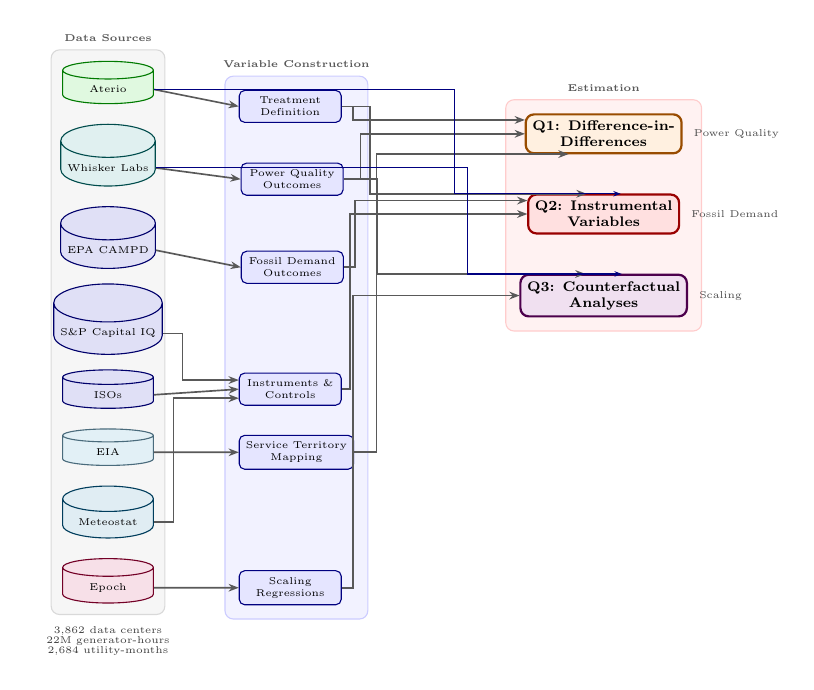
\begin{tikzpicture}[
    scale=0.72,
    transform shape,
    node distance=0.48cm and 0.7cm,
    % === STYLES ===
    source/.style={
        cylinder,
        shape border rotate=90,
        draw=#1!60!black,
        fill=#1!12,
        text centered,
        minimum height=1.55em,
        minimum width=1.6cm,
        aspect=0.35,
        font=\tiny,
        align=center
    },
    source/.default=green,
    process/.style={
        rectangle,
        draw=blue!50!black,
        fill=blue!10,
        text centered,
        rounded corners=2pt,
        minimum height=1.35em,
        minimum width=1.8cm,
        font=\tiny,
        align=center
    },
    model/.style={
        rectangle,
        draw=#1!60!black,
        fill=#1!12,
        thick,
        text centered,
        rounded corners=3pt,
        minimum height=1.85em,
        minimum width=2.4cm,
        font=\scriptsize\bfseries,
        align=center
    },
    model/.default=red,
    arrow/.style={
        -{Stealth[scale=0.65]},
        semithick,
        color=gray!70!black
    },
    directarrow/.style={
        -{Stealth[scale=0.55]},
        color=blue!50!black,
        thin
    },
    grouplabel/.style={
        font=\tiny\bfseries,
        color=gray!70!black
    },
    annot/.style={
        font=\scriptsize,
        color=gray!60!black
    }
]

% === COLUMN 1: DATA SOURCES ===

% AI/Data Center Data (green shades)
\node[source=green!80!black] (aterio) {Aterio};

% Power Quality Data (teal shades)
\node[source=teal, below=0.35cm of aterio] (whisker) {Whisker Labs};

% Generator/Market Data (blue shades)
\node[source=blue!70!black, below=0.35cm of whisker] (campd) {EPA CAMPD};
\node[source=blue!70!black, below=0.26cm of campd] (spiq) {S\&P Capital IQ};
\node[source=blue!70!black, below=0.26cm of spiq] (isos) {ISOs};

% Government/Geographic (cyan shades)
\node[source=cyan!70!black, below=0.35cm of isos] (eia) {EIA};

% Weather (blue-green shades)
\node[source=blue!60!green, below=0.35cm of eia] (weather) {Meteostat};

% AI Model Data (purple shades)
\node[source=purple, below=0.35cm of weather] (epoch) {Epoch};

% === COLUMN 2: DATA CONSTRUCTION STEPS ===

% Treatment Definition
\node[process, right=1.5cm of aterio, yshift=-0.3cm] (treat_def) {Treatment\\Definition};

% Outcome Construction
\node[process, right=1.5cm of whisker, yshift=-0.2cm] (outcome_pq) {Power Quality\\Outcomes};

% Fossil Demand Construction
\node[process, right=1.5cm of campd, yshift=-0.3cm] (fossil_dem) {Fossil Demand\\Outcomes};

% Instrument Construction
\node[process, right=1.5cm of isos, yshift=0.1cm] (instruments) {Instruments \&\\Controls};

% Service Territory Mapping
\node[process, right=1.5cm of eia] (territory) {Service Territory\\Mapping};

% Scaling Data
\node[process, right=1.5cm of epoch] (scaling) {Scaling\\Regressions};

% === COLUMN 3: ANALYSIS MODELS ===

% Q1: DiD Model
\node[model=orange, right=3.2cm of outcome_pq, yshift=0.8cm] (q1) {Q1: Difference-in-\\Differences};

% Q2: IV Model  
\node[model=red, below=0.7cm of q1] (q2) {Q2: Instrumental\\Variables};

% Q3: Counterfactual Model
\node[model=violet, below=0.7cm of q2] (q3) {Q3: Counterfactual\\Analyses};

% === CONNECTIONS ===

% To Treatment Definition
\draw[arrow] (aterio.east) -- (treat_def.west);

% To Power Quality Outcomes
\draw[arrow] (whisker.east) -- (outcome_pq.west);

% To Fossil Demand Outcomes
\draw[arrow] (campd.east) -- (fossil_dem.west);

% To Instruments & Controls
\draw[arrow] (spiq.east) -- ++(0.35,0) |- (instruments.170);
\draw[arrow] (isos.east) -- (instruments.west);
\draw[arrow] (weather.east) -- ++(0.35,0) |- (instruments.190);

% To Service Territory Mapping
\draw[arrow] (eia.east) -- (territory.west);

% To Scaling Regressions
\draw[arrow] (epoch.east) -- (scaling.west);

% === CONNECTIONS TO MODELS ===

% Q1 connections
\draw[arrow] (treat_def.east) -- ++(0.2,0) |- (q1.170);
\draw[arrow] (outcome_pq.east) -- ++(0.3,0) |- (q1.west);
\draw[arrow] (territory.east) -- ++(0.4,0) |- (q1.210);

% Q2 connections
\draw[arrow] (treat_def.east) -- ++(0.5,0) |- (q2.130);
\draw[arrow] (fossil_dem.east) -- ++(0.2,0) |- (q2.170);
\draw[arrow] (instruments.east) -- ++(0.15,0) |- (q2.west);

% Q3 connections
\draw[arrow] (outcome_pq.east) -- ++(0.6,0) |- (q3.130);
\draw[arrow] (scaling.east) -- ++(0.2,0) |- (q3.west);

% Direct data feeds
\draw[directarrow] (aterio.east) -- ++(5.3,0) |- (q2.50);
\draw[directarrow] (whisker.east) -- ++(5.5,0) |- (q3.50);

% === BACKGROUND GROUPINGS ===
\begin{scope}[on background layer]
    % Raw Data Sources
    \node[fit=(aterio)(epoch), 
          fill=gray!7, 
          rounded corners=3pt, 
          draw=gray!30,
          inner sep=4pt] (rawbox) {};
    \node[grouplabel, above=0.02cm of rawbox.north] {Data Sources};
    
    % Data Construction
    \node[fit=(treat_def)(scaling)(territory)(instruments), 
          fill=blue!5, 
          rounded corners=3pt, 
          draw=blue!20,
          inner sep=5pt] (constructbox) {};
    \node[grouplabel, above=0.02cm of constructbox.north] {Variable Construction};
    
    % Models
    \node[fit=(q1)(q2)(q3), 
          fill=red!5, 
          rounded corners=3pt, 
          draw=red!20,
          inner sep=5pt] (modelbox) {};
    \node[grouplabel, above=0.02cm of modelbox.north] {Estimation};
\end{scope}

% === ANNOTATIONS ===
% Observation counts
\node[font=\fontsize{4}{5}\selectfont, color=gray!50!black, below=0.08cm of rawbox.south, text width=2.6cm, align=center] 
    {3,862 data centers\\22M generator-hours\\2,684 utility-months};

% Model annotations
\node[annot, right=0.08cm of q1.east] {\tiny Power Quality};
\node[annot, right=0.08cm of q2.east] {\tiny Fossil Demand};
\node[annot, right=0.08cm of q3.east] {\tiny Scaling};

\end{tikzpicture}
\caption{Data sources and analysis pipeline. Data sources flow through variable construction into three estimation strategies addressing power quality impacts (Q1), fossil fuel demand (Q2), and counterfactual scaling scenarios (Q3).}
\label{fig:DataDiagram}
\end{figure}


%\niranjan{This following paragraph can be compressed since we detail the sources under 5.2 anyway. Just keep the first line and toss the rest. If there are additional pieces of information here then merge them into 5.1 and 5.2 as appropriate.}
 %Weather data come from \textbf{Meteostat}, which reports hourly temperature and precipitation; fuel cost data are obtained from \textbf{S\&P Capital IQ Global}, which publishes historical natural gas price series; and generator-level demand and heat rate data are published by the \textbf{EPA} through the Continuous Air Monitoring and Power Data (CAMPD). In addition, we construct zonal market boundaries using maps provided by \textbf{U.S. Independent System Operators (ISOs)} and merge these with ISO wholesale price data. Finally, we use geographic service territory files from the \textbf{EIA} to ensure consistent alignment of generator-, zonal-, and retail-level observations across datasets.  
\subsection{Variables of Interest}
%\niranjan{separately specify the variables of interest and the data needed for each question here. call them out explicitly with bold face or italics or some headings.}

We use three primary datasets. First, the \textbf{Consumer Power Quality Index (CPQI)} from \cite{WhiskerLabs_THD_2024} provides a composite measure of consumer-facing reliability events (surges, sags, brownouts, interruptions), summarizing frequency and severity of power deviations at the household level. Second, \textbf{Total Harmonic Distortion (THD)} data from \cite{WhiskerLabs_THD_2024} offers a \emph{technical measure of waveform distortion}, quantifying voltage deviation from a clean 60-Hz sine wave. Elevated THD indicates grid stress, reduces motor efficiency, and shortens equipment lifespan. Figure \ref{fig:THD} illustrates how harmonics alter voltage sine waves, reducing power reliability. Since THD data are more recent than CPQI, fewer model releases are available for THD analysis. Finally, we incorporate \textbf{generator demand} from EPA's CAMPD database, providing \emph{hourly plant-level demand} that captures local operating characteristics. CAMPD data span 2021--2023, constraining analysis to AI model releases within that period.
\subsection{Control Variables}

For the \textbf{power quality regressions}, we use a parsimonious specification with only time and geographic fixed effects, which absorb seasonal patterns, long-run trends, and location-specific differences, allowing us to test whether data center activity coincides with reliability declines beyond geography and time. In contrast, the \textbf{generator demand regressions} employ a richer set of controls to address endogeneity, using \emph{generator heat rates} from EPA CAMPD and \emph{natural gas prices} from S\&P Capital IQ Global as instruments in a two-stage least squares framework, along with CAMPD’s hourly generator demand data (2021–2024). We also incorporate \emph{Meteostat} weather variables (temperature, dewpoint, precipitation) to capture demand and renewable variability, and \emph{ISO} market data based on boundary maps to ensure spatial consistency. Finally, \emph{EIA retail service territory files} reconcile generator-, zonal-, and retail-level observations into a consistent framework.


% For the \textbf{power quality regressions}, we deliberately keep controls parsimonious. Because the areas for which power quality is measured are much larger and the available dataset is significantly smaller, we restrict the specification to time and geographic fixed effects. These absorb broad seasonal patterns, long-run trends, and location-specific differences that could confound observed changes in power quality. We do not include fuel or generator-level variables here, because the goal is to isolate whether data center activity coincides with localized deteriorations in reliability beyond what is explained by geography and time.  


% In contrast, for the \textbf{generator demand regressions}, we employ a richer set of external data sources to address the endogeneity of prices and generation. In particular, we use \emph{generator heat rates} from the EPA’s Continuous Air Monitoring and Power Data (CAMPD) and \emph{natural gas price series} from S\&P Capital IQ Global as instruments in a two-stage least squares framework. Heat rates capture technological efficiency at the unit level, while natural gas prices reflect exogenous shifts in input costs; both provide valid sources of variation to predict electricity prices without being directly affected by AI model releases. The CAMPD data also supply hourly generator demand observations (2021--2024), which we use as the dependent variable in these regressions.

% We further incorporate \emph{Meteostat weather data}---hourly temperature, dewpoint, and precipitation---to capture demand fluctuations and renewable output variability, and \emph{Independent System Operator (ISO)} market data to ensure spatial and market consistency. The ISO zonal datasets are constructed by us based on geographic boundary maps provided directly by ISOs. Finally, we supplement these with \emph{EIA retail service territory files}, which we use to reconcile generator-, zonal-, and retail-level observations into a consistent spatial framework.  

\subsection{Combining Data Sources}
%\niranjan{Add a few lines about how these sources are combined for the problems at hand.}

To integrate datasets, we harmonize spatial and temporal units across sources. Data center locations from Aterio are mapped to ISO zones, EIA territories, and counties, enabling linkage with Whisker Labs reliability indexes (CPQI and THD) and CAMPD generator demand. CPQI has 2,683 observations (mean 0.52, s.d. 0.42), while THD is more dispersed (mean 1.81, s.d. 6.77). CAMPD generator demand averages 218 MW (s.d. 158), and wholesale prices average \$51/MWh (s.d. 148). Weather data capture local conditions (mean temperature 17°C, precipitation 0.12 mm), and time series are aligned at hourly or monthly resolution. External controls—natural gas prices, weather, and ISO market data—are merged by geography and time, yielding a unified panel suitable for difference-in-differences and IV regressions.

Our demand model focuses on deregulated markets in the Eastern Interconnection and ERCOT, where data on zones and prices are readily available, while our power quality model draws on Whisker Labs data from 72 retail utilities nationwide (monthly, 2022–2025). The demand regressions use hourly data for several thousand generators (2021–2023). We concentrate on hyperscaler AI companies—including Meta, Microsoft, Amazon, and Google—with Anthropic linked to Google due to its cloud partnership. Appendix materials include maps, sample descriptions, and data tables.


%\aruna{This is good in that it describes where we get our data very clearly, but it is still not clear which of the data we actually use---specific region, specific time interval, specific companies etc}
% \begin{table}[htbp]
% \centering
% \caption{Data sources used for each analysis question.}
% \label{tab:DataSources}
% \begin{threeparttable}
% \begin{tabularx}{\linewidth}{lXl}
% \toprule
% \textbf{Source} & \textbf{Content} & \textbf{Use in Analysis} \\
% \midrule
% \multicolumn{3}{c}{\textbf{Q1: Difference-in-Differences (Power Quality)}} \\
% \midrule
% Aterio & Data center locations, history, ownership, capacity (MW) & Define treatment regions; link AI model releases \\
% Whisker Labs & CPQI (consumer reliability); THD (waveform distortion) & Outcome variables for DiD regressions \\
% Meteostat & Temperature, precipitation & Demand and renewable controls \\
% ISOs & Zonal boundaries, wholesale prices & Regional controls; market alignment \\
% EIA & Retail service territory maps & Define treatment/control boundaries \\
% \midrule
% \multicolumn{3}{c}{\textbf{Q2: Instrumental Variables (Fossil Demand)}} \\
% \midrule
% EPA CAMPD & Hourly generator demand; heat rates & Fossil demand outcome; heat rate as instrument \\
% S\&P Capital IQ & Natural gas prices & Instrument and fuel-cost control \\
% Aterio & Data center proximity to generators & Treatment near releasing-company centers \\
% Meteostat & Temperature, precipitation & Demand and renewable controls \\
% ISOs & Zonal wholesale prices & Market controls \\
% \midrule
% \multicolumn{3}{c}{\textbf{Q3: Counterfactual Analyses (Scaling \& Efficiency)}} \\
% \midrule
% Whisker Labs & CPQI; THD & Baseline power quality impacts for scaling projections \\
% Epoch & Model parameters, FLOPs, release dates & Scaling regressions; efficiency counterfactuals \\
% GPU Experiments & Energy use with varying GPU counts/sizes & Extrapolate to production models \\
% \bottomrule
% \end{tabularx}
% \end{threeparttable}
% \end{table}
%Figure \ref{fig:PPAbyResource} shows the growth of PPAs by resource type between 2016 and 2024. Note that the amount of generation contracted has grown exponentially and that the mix of generation types has shifted from purely wind to a majority from solar with some non-renewable generation such as storage now contracted as well. 

% \begin{figure}
%     \centering
%     
\includegraphics[width=0.75\linewidth]{Figures/PPA by Resource Type.png}
%     \caption{Data Center PPAs by Resource Type}
%     \label{fig:PPAbyResource}
% \end{figure}

% \begin{figure}
%     \centering
%     
\includegraphics[width=0.5\linewidth]{Figures/Data Center Power Demand vs Green Generation.png}
%     \caption{Data Center Power Consumption vs Green Generation. Source: Aterio.io}
%     \label{fig:DCPowerConsumption}


\section{Results}

%\subsection{Econometric Results}
%\niranjan{1. Add a note on the statistical significance of the corresponding effects in each subsections.}
% \niranjan{2. For every interpretation you provide please have some data source that you used to provide that interpretation. The appendix should have expanded text that describes how that interpretation was arrived at. For example when we say 1 outage/year to 1.5-2 outages per year for the average customer, we should clearly specify which data source was used and in the appendix also show the actual calculations that we use to arrive at that specific interpretation. Provide citations to the data sources as well.}
\subsection{Power Quality Impacts}
Figure \ref{fig:powerqualityOverTime} shows the estimated impact of the release of various AI models on the local consumer power quality index (CPQI) as measured by Whisker Labs over time. The DiD coefficients (on the y-axis) represent the difference between the change in CPQI in retail electric zones with hyperscaler data centers and the change in CPQI in zones without following the release of the corresponding AI models. Higher values for the coefficients indicate deterioration in power quality that is causally attributable to the AI model releases (modulo the exhaustiveness of the controls modeled). Most coefficients are positive and significant at the 1\% level with several negative but mostly insignificant coefficients.

%\niranjan{Explain what the CPQI denotes and its typical range and then explain how 0.32 is a big bad change.} 
The CPQI is an index of the expected number of surges, power outages, and brownouts weighted by the impact of the event on the home. It typically ranges from 0 to 1.2 with higher values indicating worse power quality. The most recent yearly national average CPQI was .69 with a $.45$ standard deviation of the power quality index distribution in U.S. \textbf{The GPT-4.5 release had an estimated power quality index impact of .327.} This level of deterioration in CPQI corresponds to moving from a typical U.S. area toward the bottom quartile of power quality—roughly \textbf{the difference between $\sim$ 1 outage/year and $\sim$ 1.5–2 outages/year for the average customer}\footnote{These are calculated based on Whisker Labs description of the CPQI Score with a description of derivation in the appendix.}—and implies more frequent voltage anomalies that make motors and electronics run less efficiently and age faster.

Further, the continued scaling of AI models signals persistent and worsening impacts on power quality. As models grow and queries rise, these effects intensify. If the trend holds, areas near data centers may face a one standard deviation drop in power quality within a few years, implying over one day of outages annually—far above the engineering standard of one outage every ten years \cite{NARUC_1in10_standard_ResourceAdequacy}. While off-peak periods in Spring and Fall may mask deterioration, regions like the Southern U.S. and PJM—already strained by summer heat—could experience outages exceeding one per month, heightening grid stress and risks of widespread failures \cite{NERC_2025_Summer_Reliability_Assessment,Thompson2024_AI_Datacenters_Energy_Dynamics}, as current Whisker Labs outage data suggest.
%Note the increase in the effect on power quality as time as gone on. A higher value represents worse power in a particular retail power authority area with a standard deviation of power quality of .45. The results indicate that large frontier models released by Google, Microsoft, and Facebook are consistently associated with statistically significant hits to power quality. GPT-4.5 had a power quality index impact of .327. A .327 deterioration in CPQI corresponds to moving from a typical U.S. area toward the bottom quartile of power quality—roughly the difference between $\sim$ 1 outage/year and $\sim$ 1.5–2 outages/year for the average customer—and implies more frequent voltage anomalies that make motors and electronics run less efficiently and age faster.

\begin{figure}[t!]
    \centering
    % First figure
    \begin{minipage}[t]{0.45\linewidth}
        \centering
        
\includegraphics[width=\linewidth]{Figures/Impact of AI on Power Quality Over Time.png}
        \caption{Impact of selected AI models on power quality over time. Plot shows substantial deterioration in power quality for recent models.}%\niranjan{Let's also add a line for half-standard deviation. We could try a separate plot where we could show the power quality drop relative to the average power quality in each models specific retail zone. Would this make sense?} %\niranjan{Please increase font sizes for this plot though.}
        \label{fig:powerqualityOverTime}
    \end{minipage}
    \hfill
    % Second figure
    \begin{minipage}[t]{0.45\linewidth}
        \centering
        
\includegraphics[width=\linewidth]{Figures/ModelEffectPowerQuality.png}
        \caption{Impact of selected AI models on Whisker Labs' total harmonic distortions metric over Time. Plot shows increasing impact over time.}
        \label{fig:THDChange}
    \end{minipage}
\end{figure}

Figure \ref{fig:THDChange} shows how larger AI models increase Harmonic Frequency deviations in retail electric zones with hyperscaler data centers compared to zones without. Claude 3.7 Sonnet and GPT 3.5 both worsen the Total Harmonic Distortion (THD) index by .436, pushing neighborhoods from safe power limits to dangerous levels. This increase causes home appliances like refrigerators and air conditioners to run hotter and less efficiently, potentially halving their lifespan \cite{IEEE519_2014,LaughnerEtAl_2024_THDonUSGrid}. The pattern indicates that larger commercial AI model deployments correlate with measurable power quality degradation, increasing consumer costs and straining the electrical grid.

% Figure \ref{fig:THDChange} shows the impacts of specific larger models on the proportion of Harmonic Frequency deviations. The coefficients represent the change in the Whisker Labs Total Harmonic Distortion (THD) index following the release of the AI model in retail electric zones with data centers owned by hyperscalers compared to the change in zones without. \textbf{Claude 3.7 Sonnet and GPT 3.5 both achieve a worsening of the total harmonic frequency metric of .436}. A .436 increase in THD is akin to taking a neighborhood that usually runs just under the safe limit for power waveform distortion and pushing it well past that limit—enough that \textbf{many homes would see refrigerators, air conditioners, and compressors run hotter and less efficiently, potentially halving their useful lifespan compared to what they would get under cleaner power} based on examination provided by \cite{IEEE519_2014} and \cite{LaughnerEtAl_2024_THDonUSGrid}. Overall, the pattern suggests that the release of increasingly large and commercially deployed models is correlated with measurable local impacts on power quality. These impacts will lead to higher costs to consumers and further strain an already fragile grid.
%, with Google’s and Microsoft’s models driving much of the explanatory power, and Facebook’s Llama 4 contributing comparably at scale.




% \vspace{.2cm}

% Tables \ref{DIDTotal}, \ref{DIDGas}, and \ref{DIDNGInteract} show the impacts of a data center’s announcement on the interconnection queue generally and for natural gas specifically. Both the overall queue length and the natural gas queue length increase following data center announcements, and the effects are larger for bigger data centers. In the specification interacting announcements with data center capacity, the results imply that each megawatt (MW) of announced data center capacity is associated with roughly 0.32 MW of additional natural gas queue capacity. This effect remains positive and significant even with county and year fixed effects. In contrast, the total interconnection queue also expands following announcements—by more than 700 MW without fixed effects, and about 150 MW with fixed effects. Taken together, these results suggest that new data centers are associated with a substantial extension of the interconnection queue, and that natural gas projects in particular are disproportionately added to the queue in anticipation of future demand.

\subsection{Power Demand Effects}
Figures \ref{fig:powerForInference} and \ref{fig:powerForTraining} visualizes our estimates of changes in power usage in MWh in the first three months before and after the release of specific large language models respectively. The pre-treatment coefficients reflect power usage (i.e. demand) of training the models, and post-treatment ones reflect that of inference. 
% \begin{wrapfigure}{r}{0.45\linewidth}
%     \vspace{-10pt}
%     
\includegraphics[width=\linewidth]{Figures/Aggregate Impacts Models.png}
%     \caption{Increase in fossil fuel electricity demand surrounding model release.\niranjan{separate training and inference}}%\niranjan{Let's organize this by increasing model size.}}%\niranjan{increase font size.}}
%     \label{fig:DiDDemand}
%     \vspace{-10pt}
% \end{wrapfigure}

\begin{figure}[t!]
    \centering
    % First figure
    \begin{minipage}[t]{0.45\linewidth}
        \centering
        
\includegraphics[width=\linewidth]{Figures/Aggregate Demand Training.png}
        \caption{Impact of selected AI models on power demand for training.}
        \label{fig:powerForInference}
    \end{minipage}
    \hfill
    % Second figure
    \begin{minipage}[t]{0.45\linewidth}
        \centering
        
\includegraphics[width=\linewidth]{Figures/Aggregate Demand Inference.png}
        \caption{Impact of selected AI models on power demand for inference.}
        \label{fig:powerForTraining}
    \end{minipage}
\end{figure}
The estimates represent the \textbf{aggregate difference between the change in the demand for generators in the ten square miles surrounding data centers compared to other areas after accounting for controls.} We see substantial increases in power demand significant at the 1\% level both during training (pre-treatment), and inference (post-treatment) as shown by the large coefficient values for most models. The smaller coefficients found for some models (both positive and negative) are not statistically significant. 

The largest effect on power demand is in the order of terawatt hours (i.e. millions of megawatt-hours). GPT-3.5 and DALL-E, for instance, are estimated to have increased aggregate electricity demand by \textbf{over one million and nearly three million megawatt-hours} respectively in the post-treatment period. To put this into perspective, the average U.S. household consumes about 10 to 11 megawatt-hours per year according to \cite{USHouseholdConsumption}. This means the additional electricity demand attributable to GPT-3.5 in the three months post release is roughly equivalent to powering \textbf{100,000 homes for a full year}, while the impact of DALL-E corresponds to nearly \textbf{300,000 homes’ annual electricity use}. These changes represent the net effects of the model release including both adoption and use of models by the public. %\niranjan{Note that these are assertions based on the net effect of the model release which also includes the adoption and use of these models by the public.}

%In validation of our metric, public-facing models such as GPT-3.5 and DALL-E used more compute for inference while larger models use more compute for training\footnote{\niranjan{While there are common factors that affect both training and inference power such as model size and computation per input, there are many that are specific to each. For example, training is largely affected by the size of training data, the optimization algorithm, and other details of the training strategy. Inference power usage on the other hand depends on the number of queries issued to the model. Specific comparisons between training and inference trends will require carefully accounting for differences in these factors.}} . 
% \dana{I think we just drop this paragragh. I get the sense the point I am trying to make is weaker than it should be to be worth keeping it.}\niranjan{I dont understand how this is validating our metric? It is not necessarily a known fact that 3.5 and DALL-E spent more compute on inference relative to training. If there are sources that support this, let's cite them.} \niranjan{Also say something about switch and metapseudo labels.}


%These comparisons highlight how even inference-heavy models, which are ostensibly lighter than the very largest training runs, can exert electricity demands on the scale of mid-sized American cities.


\subsection{Counterfactual Analyses}

% \begin{figure}[t]
%     \centering
%     % First figure
%     \begin{minipage}[t]{0.48\linewidth}
%         \centering
%         
\includegraphics[width=\linewidth]{Figures/Model Coefficients v Power Quality.png}
%         \caption{Log model size vs. power quality impact.}
%         \label{fig:ModelSizeandPowerQuality}
%     \end{minipage}
%     \hfill
%     % Second figure
%     \begin{minipage}[t]{0.48\linewidth}
%         \centering
%         \includegraphics[width=\linewidth]{Figures/ModelSizePowerDrawComparison.png}
%         \caption{Impacts of increasing GPUs and model size on power consumption.}
%         \label{fig:ModelSizeTechnicalData}
%     \end{minipage}
% \end{figure}

%\begin{wrapfigure}{r}{0.45\linewidth}
%    \vspace{-10pt} % adjust vertical position relative to the text
%    \centering
%    
\includegraphics[width=0.90\linewidth]{Figures/Model Coefficients v Power Quality.png}
%    \caption{Log model size vs. power quality impact.}
%    \label{fig:ModelSizeandPowerQuality}
%    \vspace{-10pt} % tighten space below caption
%\end{wrapfigure}

%The results above show that scaling--increasing model size and training--leads to measurable power quality deterioration and large increases in power demand. Here we show two examples of counterfactual analyses that we can conduct based on the data and models we have developed.
Here we show an example of a counterfactual analysis that we can conduct based on the data and models we have developed. In particular, we can combine data on model size (i.e. parameter counts) and our estimates of power quality and demand to fit separate trend lines. We can then use these trend lines to extrapolate power quality impacts and demand change at other model sizes. Specific regression details in terms of model-fit and coefficient values can be found in the appendix.

To illustrate this we fit a line to power quality impacts of three models: Llama-3.1 (405 B), PaLM (540B), and Llama 4 Behemoth (2T). 
Using this line we see that going from a 2 Trillion model (the largest in our data set) to say a 4 Trillion model would result in a change in power quality impact from \textbf{0.321 to 0.434}, a deterioration of about 0.113 units, or just over 35 percent relative to the 2 trillion baseline. Furthermore, the relationship is exponential (the line is over log parameter counts), so a 100 billion parameter decrease has a more significant percentage-wise impact at 400 Billion parameters than at 800 Billion. The larger models become, the greater the required decrease in parameters for the same percentage decrease in power quality impact.

Using a similar process as above, we also extrapolate demand. We find that \textbf{each 1\% parameter increase leads to 0.15\% higher power demand} within three months of model release. Scaling from say 540 billion to one trillion parameters would \textbf{increase total power demand by 10.5\%}. For DALL-E, halving parameters would \textbf{reduce inference demand by $\sim$300 GWh}, equivalent to the annual consumption of \textbf{27--30 thousand homes.}

Training compute requirements also have measurable effects: a one percent increase in FLOPs is associated with a \textbf{.1 percent increase in power demand}. For GPT-3.5, halving training compute FLOPs is equivalent to reducing usage by enough energy to power \textbf{8 to 10 thousand US homes for a year.} Other counterfactuals could be performed including regressing inference coefficients on reported model queries to determine the scaling effect of additional queries on model demand or determining the impacts of changing model size on carbon emissions based on the emissions mix from the data.
%the annual output of a 48 MW solar plant. 

%Finally, Figure \ref{fig:ModelSizeTechnicalData} shows experimental results from lab-based experiments in running smaller AI models on GPUs. Energy usage by AI model is provided as the full bar with the light portion representing message passing. \niranjan{This has not been published, so we need to provide additional details on this setup.} These results show that message passing consumes between 14 and 41 percent of inference power. Reducing this cost by half would cut total inference energy by about seven percent. For Google’s Minerva (540B) model, this would correspond to \textbf{a reduction of 96 GWh}, enough energy to cover a fleet of roughly 4,800–6,000 electric vehicles annual driving needs. These results should be interpreted as approximate, since they rely on a limited number of models, but they highlight the importance of model design choices for grid outcomes.
%\niranjan{Aruna and Dana, I am wondering if we should drop figure 9 and its discussion here. We should instead use results from other published studies on energy estimates. }
% We run counterfactual analyses to illustrate the impacts of AI efficiency on power quality and power demand. We combine our econometric estimates with data from the Epoch database on the number of parameters of models as well as estimates of the impacts of increasing model parameters on relative energy usage. Figure \ref{fig:ModelSizeandPowerQuality} shows the relationship between model parameters and the coefficients on the power quality index by particular models. One trillion additional parameters in an LLM model is associated with a third of a standard deviation drop in power quality. If the progression from a 100-billion-parameter model to a one-trillion-parameter model brings with it a one-third standard deviation hit to power quality, this is comparable to additional mid-sized city’s worth of highly variable industrial load. This reframes model growth not just as a compute challenge, but as a grid-reliability issue. Further, a doubling parameters is associated with about a 0.056 point increase in CPQI or 12\% of a standard deviation. This means that going from a 175 Billion parameter model to a 350 Billion parameter model could meaningfully impact household distortion experience.


% Using the power demand results, a one percent increase in parameters leads to a .15 percent increase in power demand in the three months after publication. Increasing model size from 540 billion parameters to 1 trillion parameters is predicted to increase total power demand by about 10.5\%. For a model like DALL-E, reducing the number of parameters by half is predicted to lead to a drop in inference power usage of 300 GW in the treatment time period or roughly the yearly output of $\sim$ 32 utility-scale wind turbines. The Epoch dataset also has information on training compute flop. A one percent increase in training compute flop is associated with a .1 percent increase in total power demand to generators near a data center prior to the publication of a model. This means that for GPT-3.5, halving the training compute flop would be associated with a decrease in power usage or roughly the annual production of a $~$ 48 MW utility-scale solar plant. It should be noted that these analyses rely on limited sample sizes in terms of number of models and should be treated like rough estimates of the effects of changes in model design.

% We further perform 

% We also perform a techno-economic analysis of the impacts of increasing model size and number of simultaneous GPUs on energy consumption. The type of analysis combines the econometric estimates with experiments we have conducted on the impacts of changing details of models. Figure \ref{fig:ModelSizeTechnicalData} shows the results of experiments with a subset of small models. Models are compared based on Watt hours for training on different numbers of GPUs and different sizes. This provides experimental data on the relative energy costs of increasing model size and GPUs to train. Increasing simultaneous GPUs is both costly in terms of running multiple machines simultaneously and also in terms of message passing, which is shown in the lighter color for the bars. Message passing between GPUs utilizes between 14 and 41 percent of training power. Using 14 percent as a lower-end estimate, this implies that reducing the cost of message passing by half would lead to a 7 percent reduction in power consumption by a model in training. For model Meta Pseudo Labels released by Google, this would imply a drop in training power consumption of 288 GWh or the equivalent of keeping a 33 MW industrial load completely off the grid for a year.


%We combine our econometric estimates of AI model's impacts on power quality and power demand with estimates from the literature on the impacts of efficiency speedups on relative energy usage. This allows us to make calculations for how much energy would decrease if specific efficiency improvements were made to AI models.

\section{Conclusion}

Understanding how AI models impact U.S. power grids is critical for ensuring energy reliability and security. This work introduces an econometric methodology to overcome the lack of fine-grained data about contributing factors. In particular, we use a difference-in-differences regressions to provide econometric estimates of the amount of power being used by specific AI models as well as the power distortions being caused by AI. We find evidence that AI is making power quality significantly worse and increasing fossil fuel power demand. We provide estimates of the potential impacts of increasing efficiency of AI on the power draw of data centers.

Our approach differs from the approach traditionally taken by the computer science energy efficiency literature, which tends to focus on the micro-scale to build up estimates of the costs of training a model in a specified way a specified number times. Our estimates of power demand impacts are significantly higher than previous literature estimates. Our approach also differs from the current approach amongst energy economists who tend to utilize changes from baseline simulation models to determine the impacts of external demand shocks. By focusing on market data, our approach is able to achieve estimates that are in between these levels of analysis. Our estimation is able to agnostically consider all electricity adds from AI model activities, which provides a more realistic estimate of AI life-cycle power demand. We believe this approach is also applicable for other other opaque impacts—such as the effect of large model releases on network congestion or cooling water demand—wherever direct usage data from providers is inaccessible.



%Our methodological contribution is portable beyond the specific case of AI and electricity. By combining econometric causal inference (difference-in-differences, instrumental variables) with domain-specific data sources, we establish a general toolkit for quantifying hidden infrastructure externalities of AI systems. The same design could be adapted to study other opaque impacts—such as the effect of large model releases on network congestion, semiconductor supply chains, or cooling water demand—whenever direct usage data from providers are inaccessible. In this sense, our approach provides a scalable, data-efficient way for AI researchers to infer systemic costs and reliability effects, complementing simulation-based analyses in computer science with causal identification strategies from economics.

While informative, this approach inherits the limitations of all Difference-in-Differences experimental designs. It relies on the parallel trends assumption, which may be violated if treated and control regions were already diverging or if generators anticipated model releases. %Spillovers across regions and heterogeneous impacts by grid or model type can further bias estimates.
Timing is also critical—effects may emerge gradually or with lags, complicating interpretation. Finally, contemporaneous shocks such as weather or other industrial expansions can confound results, and the treatment itself (a model release) may not map cleanly onto actual deployment. Ideally, we would like a longer power quality dataset with more granularity to make cleaner statements about long-term trends.

\bibliography{Energy}

\appendix
\appendix
\section{Appendix}
\subsection{Total Harmonic Distortion}
\begin{wrapfigure}{r}{0.3\linewidth}
    \centering
    \vspace{-18pt}
    
\includegraphics[width=\linewidth]{Figures/HarmonicDistortion.png}
    \caption{Total harmonic distortion representation.}%\aruna{this figure is not referenced in the text}}        
    \label{fig:THD}
    \vspace{5pt}
\end{wrapfigure}
Figure~\ref{fig:THD} illustrates the distortions in the power frequencies. The green lie shows the \emph{clear} voltage curve, which is cleanly sinusoidal, whereas with huge loads can produce harmonic distortions shown as the dotted yellow curve. This \emph{dirtier} voltage can adversely affect the operation and lifetime of household appliances and other products that use electricity.
\newpage

\subsection{Results Tables}

\begin{table}[hbp]
\centering
\caption{Estimated Impact of AI Model Releases on Power Quality}
\label{tab:AIModelsPowerQuality}
\small
\begin{tabular}{l l r r r}
\toprule
Model & Provider & Coefficient & Std. Error & $R^{2}$ \\
\midrule
GPT-4.5                  & Microsoft   & 0.327*** & 0.087 & 0.327 \\
Llama 4 Behemoth (preview) & Facebook  & 0.325*** & 0.074 & 0.313 \\
Claude 3 Opus            & Google      & 0.278*** & 0.043 & 0.462 \\
Gemini 1.5 Pro           & Google      & 0.223*** & 0.026 & 0.451 \\
GPT-4o                   & Microsoft   & 0.198*** & 0.044 & 0.331 \\
GPT-4                    & Microsoft   & 0.176*** & 0.033 & 0.408 \\
Claude 3.7 Sonnet        & Google      & 0.161*** & 0.041 & 0.357 \\
Chinchilla               & Google      & 0.143*** & 0.038 & 0.570 \\
PaLM (540B)              & Google      & 0.142*** & 0.029 & 0.587 \\
LaMDA                    & Google      & 0.134**  & 0.044 & 0.564 \\
PaLM 2                   & Google      & 0.133*** & 0.024 & 0.465 \\
Claude 3.5 Sonnet        & Google      & 0.126*** & 0.036 & 0.378 \\
OPT-175B                 & Facebook    & 0.104*** & 0.023 & 0.467 \\
Gemini 1.0 Ultra         & Google      & 0.103*** & 0.021 & 0.409 \\
Llama 3.1-405B           & Facebook    & 0.052    & 0.034 & 0.315 \\
Minerva (540B)           & Google      & 0.031    & 0.023 & 0.519 \\
Parti                    & Google      & 0.031    & 0.023 & 0.519 \\
GPT-4 Turbo              & Microsoft   & 0.030*   & 0.017 & 0.308 \\
GPT-3.5                  & Microsoft   & -0.049** & 0.018 & 0.390 \\
Flan-PaLM 540B           & Google      & -0.051*  & 0.026 & 0.508 \\
U-PaLM (540B)            & Google      & -0.051*  & 0.026 & 0.508 \\
Amazon Titan             & Amazon AWS  & -0.086***& 0.016 & 0.380 \\
\bottomrule
\end{tabular}
\begin{flushleft}
\footnotesize
Notes: Robust standard errors in parentheses. Significance levels: *** $p<0.01$, ** $p<0.05$, * $p<0.1$.
\end{flushleft}
\end{table}

\begin{table}[htbp]\centering
\caption{Difference-in-Differences Estimates of Data Center Announcements on Cumulative Total Queue Capacity (MW)}
\begin{threeparttable}
\begin{tabular}{lcc}
\toprule
& (1) & (2) \\
& No FE & County \& Year FE \\
\midrule
Post Announcement & 714.459\sym{**} & 150.741\sym{*} \\
& (293.890) & (87.001) \\
Intercept & 366.406\sym{***} & -188.142\sym{***} \\
& (19.361) & (13.395) \\
\midrule
Observations & 128,700 & 128,700 \\
R$^2$ & 0.010 & 0.780 \\
Adj.\ R$^2$ & 0.010 & 0.777 \\
Fixed Effects & No & County \& Year \\
\bottomrule
\end{tabular}
\begin{tablenotes}[flushleft]
\footnotesize
\item Cluster-robust standard errors in parentheses. 
\item \sym{*} $p<0.10$, \sym{**} $p<0.05$, \sym{***} $p<0.01$. 
\end{tablenotes}
\end{threeparttable}
\label{DIDTotal}
\end{table}

\begin{table}[htbp]\centering
\caption{Difference-in-Differences Estimates of Data Center Announcements on Cumulative Gas Queue Capacity (MW)}
\begin{threeparttable}
\begin{tabular}{lcc}
\toprule
& (1) & (2) \\
& No FE & County \& Year FE \\
\midrule
Post $\times$ Announced Capacity & 0.324\sym{***} & 0.250\sym{**} \\
& (0.105) & (0.117) \\
Intercept & 175.718\sym{***} & -43.457\sym{***} \\
& (18.388) & (13.229) \\
\midrule
Observations & 16,380 & 16,380 \\
R$^2$ & 0.012 & 0.610 \\
Adj.\ R$^2$ & 0.012 & 0.604 \\
Fixed Effects & No & County \& Year \\
\bottomrule
\end{tabular}
\begin{tablenotes}[flushleft]
\footnotesize
\item Cluster-robust standard errors in parentheses. 
\item \sym{*} $p<0.10$, \sym{**} $p<0.05$, \sym{***} $p<0.01$. 
\end{tablenotes}
\end{threeparttable}
\label{DIDGas}
\end{table}

\begin{table}[htbp]\centering
\caption{Difference-in-Differences Estimates of Data Center Announcements on Cumulative Gas Queue Capacity (MW), No Interaction}
\begin{threeparttable}
\begin{tabular}{lcc}
\toprule
& (1) & (2) \\
& No FE & County \& Year FE \\
\midrule
Post Announcement & 98.976 & 273.893\sym{***} \\
& (68.413) & (79.284) \\
Intercept & 176.560\sym{***} & 63.585\sym{***} \\
& (18.656) & (1.28e-11) \\
\midrule
Observations & 16,380 & 16,380 \\
R$^2$ & 0.003 & 0.522 \\
Adj.\ R$^2$ & 0.002 & 0.514 \\
Fixed Effects & No & County \& Year \\
\bottomrule
\end{tabular}
\begin{tablenotes}[flushleft]
\footnotesize
\item Cluster-robust standard errors in parentheses. 
\item \sym{*} $p<0.10$, \sym{**} $p<0.05$, \sym{***} $p<0.01$. 
\end{tablenotes}
\end{threeparttable}
\label{DIDNGInteract}
\end{table}

% POST-TREATMENT EFFECTS
\begin{table}[htbp]
\centering
\caption{Post-Treatment: Estimated Impact of AI Model Releases on Aggregate Electricity Demand}
\label{tab:ai_demand_post}
\resizebox{\columnwidth}{!}{%
\begin{threeparttable}
\begin{tabular}{l l r r r r}
\toprule
Model & Provider & Coefficient & $p$-value & $R^{2}$ & Aggregate Impact (MWh) \\
\midrule
Switch                         & Google     & 124.46 & $<0.001$ & 0.628 & 4,154,379 \\
DALL\text{-}E                  & Microsoft  &  81.54 & $<0.001$ & 0.627 & 2,910,208 \\
GPT\text{-}3.5                 & Microsoft  &  76.08 & $<0.001$  & 0.622 & 1,034,517 \\
mT5\text{-}XXL                 & Google     &  63.48 & $<0.001$              & 0.625 &   420,630 \\
Megatron\text{-}Turing NLG 530B& Microsoft &  46.15 & $<0.001$  & 0.628 & 1,692,209 \\
Codex                          & Microsoft  &  35.60 & 0.0211                & 0.630 & 2,132,043 \\
Minerva (540B)                 & Google     &  24.03 & 0.4305                & 0.624 & 1,372,621 \\
Parti                          & Google     &  20.14 & 0.4692                & 0.625 & 1,183,787 \\
Flan\text{-}PaLM (540B)        & Google     &  17.36 & 0.0501                & 0.622 &   504,750 \\
U\text{-}PaLM (540B)           & Google     &  17.36 & 0.0501                & 0.622 &   504,750 \\
OPT\text{-}175B                & Facebook   &  12.85 & 0.0161                & 0.624 &   583,999 \\
ByT5\text{-}XXL                & Google     &   1.28 & 0.9584                & 0.624 &    66,424 \\
ProtT5\text{-}XXL              & Google     &  -1.42 & 0.9370                & 0.629 &   -64,268 \\
Meta Pseudo Labels             & Google     &  -3.996& 0.8284                & 0.628 &  -118,203 \\
FLAN 137B                      & Google     &  -4.97 & 0.7971                & 0.624 &  -167,480 \\
Chinchilla                     & Google     & -23.54 & 0.0980                & 0.628 &  -834,056 \\
PaLM (540B)                    & Google     & -24.53 & 0.0714                & 0.628 &  -873,641 \\
LaMDA                          & Google     & -27.41 & 0.1362                & 0.626 &  -643,963 \\
GLaM                           & Google     & -27.76 & 0.3485                & 0.625 &  -750,319 \\
Gopher (280B)                  & Google     & -30.32 & 0.3113                & 0.625 &  -813,756 \\
\bottomrule
\end{tabular}
\begin{tablenotes}
\item Notes: Coefficients and p-values are taken from \texttt{post\_coefficient} and \texttt{post\_p\_value}. Aggregate impact uses \texttt{post\_aggregate\_demand\_increase}.
\end{tablenotes}
\end{threeparttable}}
\label{PostTreatment}
\end{table}

% PRE-TREATMENT EFFECTS
\begin{table}[htbp]
\centering
\caption{Pre-Treatment: Estimated Impact of AI Model Releases on Aggregate Electricity Demand}
\label{tab:ai_demand_pre}
\resizebox{\columnwidth}{!}{%
\begin{threeparttable}
\begin{tabular}{l l r r r r}
\toprule
Model & Provider & Coefficient & $p$-value & $R^{2}$ & Aggregate Impact (MWh) \\
\midrule
Switch                         & Google     &  89.77 & $<0.001$ & 0.628 &   268,851 \\
DALL\text{-}E                  & Microsoft  &  66.90 & $<0.001$ & 0.627 &    43,755 \\
GPT\text{-}3.5                 & Microsoft  &  39.60 & $<0.001$             & 0.622 & 1,501,640 \\
% mT5\text{-}XXL                 & Google     &   —    & —                    & 0.625 &      —    \\
Megatron\text{-}Turing NLG 530B& Microsoft &  35.96 & 0.0138               & 0.628 & 2,088,496 \\
Codex                          & Microsoft  &  28.63 & 0.0108               & 0.630 & 1,245,855 \\
Minerva (540B)                 & Google     & -22.51 & 0.0972               & 0.624 &  -781,775 \\
Parti                          & Google     & -22.94 & 0.1056               & 0.625 &  -734,906 \\
Flan\text{-}PaLM (540B)        & Google     &  29.16 & 0.3543               & 0.622 & 1,475,972 \\
U\text{-}PaLM (540B)           & Google     &  29.16 & 0.3543               & 0.622 & 1,475,972 \\
OPT\text{-}175B                & Facebook   & -21.77 & 0.2825               & 0.624 &  -502,990 \\
ByT5\text{-}XXL                & Google     &  -6.20 & 0.7410               & 0.624 &  -177,165 \\
ProtT5\text{-}XXL              & Google     & 101.54 & $<0.001$ & 0.629 & 3,280,303 \\
Meta Pseudo Labels             & Google     & 168.29 & $<0.001$& 0.628 & 4,122,856 \\
FLAN 137B                      & Google     &   3.41 & 0.8961               & 0.624 &    181,878 \\
Chinchilla                     & Google     & -23.61 & 0.4060               & 0.628 &  -583,230 \\
PaLM (540B)                    & Google     & -22.84 & 0.4174               & 0.628 &  -554,841 \\
LaMDA                          & Google     & -27.80 & 0.3750               & 0.626 &  -817,029 \\
GLaM                           & Google     & -12.52 & 0.4856               & 0.625 &  -413,053 \\
Gopher (280B)                  & Google     &  -8.12 & 0.6566               & 0.625 &  -271,852 \\
\bottomrule
\end{tabular}
\begin{tablenotes}
\item Notes: Coefficients and p-values are taken from \texttt{pre\_coefficient} and \texttt{pre\_p\_value}. Aggregate impact uses \texttt{pre\_aggregate\_demand\_increase}. Dashes indicate missing values in the spreadsheet.
\end{tablenotes}
\end{threeparttable}}
\label{PreTreatment}
\end{table}

\newpage

\subsection{Expanded Dataset Description}

Below, maps can be found providing more detail on the data center dataset alongside tables on the datasets and the dataset sample selection criteria.

\begin{figure}
    \centering
    
\includegraphics[width=\linewidth]{Figures/Data Centers by State.png}
    \caption{Data centers by state.}
    \label{fig:placeholder}
\end{figure}

\begin{figure}
    \centering
    
\includegraphics[width=\linewidth]{Figures/ZoneMap (1).png}
    \caption{Map of zones for demand model.}
    \label{fig:placeholder}
\end{figure}

\begin{figure}
    \centering
    
\includegraphics[width=\linewidth]{Figures/THD Dataset.jpg}
    \caption{Map of Retail Electric Utilities for Whisker Labs Data.}
    \label{fig:placeholder}
\end{figure}


\begin{sidewaystable}[htbp]
\centering
\caption{Expanded description of data sources (for appendix).}
\label{tab:DataSourcesExpanded}
\resizebox{\linewidth}{!}{%
\begin{threeparttable}
\begin{tabularx}{\linewidth}{lXl}
\toprule
\textbf{Source} & \textbf{Content and Granularity} & \textbf{Use in Analysis} \\
\midrule
\multicolumn{3}{c}{\textbf{Q1: Difference-in-Differences (Power Quality)}} \\
\midrule
Aterio & Data center locations, establishment/expansion/retirement dates, ownership, and operational capacity (MW). Data are available at the facility level and updated annually. & Defines treatment regions; links AI model releases to hyperscaler-owned centers. \\
Whisker Labs & Consumer Power Quality Index (CPQI, composite measure of surges, sags, brownouts, interruptions) and Total Harmonic Distortion (THD, waveform distortion). Provided at county level, hourly frequency. & Outcome variables for DiD regressions. \\
Meteostat & Hourly temperature and precipitation, aggregated at the county level. Coverage includes all U.S. counties with weather stations. & Controls for demand fluctuations and renewable generation variability. \\
ISOs & Geographic boundary shapefiles and wholesale price data at zonal level. Boundaries digitized from ISO-provided maps; prices available hourly. & Market alignment and regional controls. \\
EIA & Retail service territory shapefiles, at utility level, updated periodically. & Used to define treatment/control boundaries and reconcile geographies. \\
\midrule
\multicolumn{3}{c}{\textbf{Q2: Instrumental Variables (Fossil Demand)}} \\
\midrule
EPA CAMPD & Hourly generator-level demand (MWh) and unit-specific heat rates (Btu/kWh). Coverage 2021--2023. & Generator demand is outcome; heat rates serve as instruments for prices. \\
S\&P Capital IQ & Daily natural gas price series, Henry Hub benchmark. National coverage. & Instrument for price and fuel-cost control. \\
Aterio & Generator proximity to data centers owned by releasing companies, matched at 10-mile radius. & Defines treatment generators in IV design. \\
Meteostat & Hourly temperature and precipitation, as above. & Controls for demand and renewable variability. \\
ISOs & Wholesale price series, zonal level, hourly frequency. & Market-level controls. \\
\midrule
\multicolumn{3}{c}{\textbf{Q3: Counterfactual Analyses (Scaling \& Efficiency)}} \\
\midrule
Whisker Labs & CPQI and THD (as above). Used to establish baseline deterioration in power quality. & Benchmark outcomes for scaling projections. \\
Epoch & AI model metadata: release dates, FLOPs, parameter counts. Public dataset with model-level detail. & Used for scaling regressions and efficiency counterfactuals. \\
GPU Experiments & Energy use measured on NVIDIA A6000 GPUs. Experiments run with batch size 4, sequence length 1024, and 200 inferences. Each bar in results represents total energy; lighter portion indicates communication overhead. Data collected in-house on 8xA6000 cluster. & Provides empirical GPU energy baselines for counterfactual scaling exercises. \\
\bottomrule
\end{tabularx}
\end{threeparttable}}
\end{sidewaystable}

\begin{sidewaystable}[htbp]
\centering
\small
\caption{Dataset sample selection and summary statistics}
\label{tab:SampleSelection}
\begin{threeparttable}
\begin{tabularx}{\linewidth}{lXl}
\toprule
\textbf{Dataset} & \textbf{Content / Summary Statistics} & \textbf{Sample Selection} \\
\midrule
Aterio & Data center locations, ownership, and capacity; mapped to ISO zones, EIA service territories, and counties & Hyperscaler data centers (Meta, Microsoft, Amazon, Google; Anthropic via Google) \\
\midrule
Whisker Labs & Reliability measures: CPQI ($N=2{,}683$, mean=0.52, s.d.=0.42); THD (mean=1.81, s.d.=6.77) & 72 retail electric utilities, monthly data 2022--2025 \\
\midrule
CAMPD & Generator-level demand: mean 218 MW (s.d.=158); operating times $\approx 1$ & Several thousand fossil generators, hourly data 2021--2023 \\
\midrule
ISOs & Wholesale electricity prices: mean $\$51$/MWh (s.d.=148); zonal boundaries & Deregulated markets in Eastern Interconnection and ERCOT \\
\midrule
Weather (Meteostat) & Temperature (mean=17°C, s.d.=11.4); precipitation (mean=0.12 mm, s.d.=0.91) & Matched by county/zone, hourly or daily resolution \\
\midrule
External Controls & Natural gas prices, ISO market data, geography/time harmonization & Used for both DiD and IV regressions \\
\bottomrule
\end{tabularx}
\begin{tablenotes}
\footnotesize
\item Notes: Time series are harmonized at hourly or monthly resolution depending on source. Unified panel supports both difference-in-differences (power quality) and instrumental variable (demand) regressions. Maps of sample regions provided in the appendix.
\end{tablenotes}
\end{threeparttable}
\end{sidewaystable}
\newpage

\subsection{Counterfactual}
Figure \ref{fig:counterQuality} shows the power quality line we fit for performing counterfactuals.

\begin{figure}
    \centering
    
\includegraphics[width=0.5\linewidth]{Figures/Power Quality Impact1.png}
    \caption{Power Quality Impact for Counterfactuals.}
    \label{fig:counterQuality}
\end{figure}

\subsection{Calculation of Comparisons}

We calculate the household average energy usage based on data provided by \cite{USHouseholdConsumption}. We simply divide our estimates by the provided numbers to get the number of households for our comparisons.

% \subsection{Robustness Checks}
% \subsubsection{Random Treatment}

% \subsubsection{Varying Spatial and Temporal Treatment Definition}



\end{document}
\endinput
%%
%% End of file `sample-sigconf-authordraft.tex'.
